%% For double-blind review submission, w/o CCS and ACM Reference (max submission space)
%\documentclass[sigplan,10pt,review,anonymous]{acmart}
%\settopmatter{printfolios=false,printccs=false,printacmref=false}
%% For double-blind review submission, w/ CCS and ACM Reference
%\documentclass[sigplan,review,anonymous]{acmart}\settopmatter{printfolios=true}
%% For single-blind review submission, w/o CCS and ACM Reference (max submission space)
%\documentclass[sigplan,review]{acmart}\settopmatter{printfolios=true,printccs=false,printacmref=false}
%% For single-blind review submission, w/ CCS and ACM Reference
%\documentclass[sigplan,review]{acmart}\settopmatter{printfolios=true}
%% For final camera-ready submission, w/ required CCS and ACM Reference
\documentclass[sigplan,nonacm,anonymous]{acmart}\settopmatter{printfolios=false,printccs=false,printacmref=false}

%% Conference information
%% Supplied to authors by publisher for camera-ready submission;
%% use defaults for review submission.
%\acmConference[ARRAY'22]{ACM SIGPLAN Conference on Programming Languages}{June 13, 2022}{San Diego, CA, USA}
%\acmYear{2018}
%\acmISBN{} % \acmISBN{978-x-xxxx-xxxx-x/YY/MM}
%\acmDOI{} % \acmDOI{10.1145/nnnnnnn.nnnnnnn}
%\startPage{1}

%% Copyright information
%% Supplied to authors (based on authors' rights management selection;
%% see authors.acm.org) by publisher for camera-ready submission;
%% use 'none' for review submission.
\setcopyright{none}
%\setcopyright{acmcopyright}
%\setcopyright{acmlicensed}
%\setcopyright{rightsretained}
%\copyrightyear{2018}           %% If different from \acmYear

\bibstyle{acmart}
\usepackage{dsfont}
\usepackage{stmaryrd}
\usepackage{colortbl}
\usepackage{hyperref}

\usepackage{amsmath}
\DeclareMathOperator*{\argmax}{argmax}
\DeclareMathOperator*{\argmin}{argmin}
\usepackage{amssymb}

\usepackage[dvipsnames, table]{xcolor}
\usepackage{textcomp}

% Packages
\usepackage[pdf]{graphviz}
\usepackage{mathrsfs}

\newcommand*\circled[1]{\tikz[baseline=-0.1cm]{
  \node[shape=circle,draw,inner sep=0.48pt] (char) {\fontsize{7}{12}\textsf{#1}};}}

\DeclareMathAlphabet{\mathcal}{OMS}{cmsy}{m}{n}
\usepackage{cancel}
\newcommand\ccancel[2][red]{\renewcommand\CancelColor{\color{#1}}\cancel{#2}}
\newcommand{\nDownarrow}{\ensuremath{\text{ }\cancel{\Downarrow}\text{ }}}
\usepackage{centernot}

\usepackage{pgfplots, pgfplotstable}
\pgfplotsset{compat=1.7}
\usepgfplotslibrary{fillbetween}
\usetikzlibrary{patterns}
\pgfmathdeclarefunction{gauss}{2}{\pgfmathparse{1/(#2*sqrt(2*pi))*exp(-((x-#1)^2)/(2*#2^2))}}
\pgfmathdeclarefunction{nil}{1}{\pgfmathparse{0.001}}

\usepackage{arydshln}
\usepackage{adjustbox}
\usepackage{enumerate}
\usepackage{enumitem}
\usepackage{tikz-cd}
\usetikzlibrary{calc}
\usepackage{amsfonts}
%\usepackage{prooftrees}
\usepackage{bussproofs}
\renewcommand{\sectionautorefname}{\S}
\renewcommand{\subsectionautorefname}{\S}
\usepackage{float}

\usepackage{tikz-3dplot}
\usetikzlibrary{3d}
\usetikzlibrary{calligraphy}
\newif\ifshowcellnumber
\showcellnumbertrue

\usepackage{algorithm}
\usepackage{algpseudocode}
\usepackage{algorithmicx}
\usepackage{sourcecodepro}
\usepackage{tikz-qtree}
\usepackage{amsthm}
\usepackage{bm}
\usetikzlibrary{bayesnet}
\usetikzlibrary{arrows}
\usepackage{subcaption}
\usetikzlibrary{backgrounds}
\usetikzlibrary{tikzmark}
\usetikzlibrary{hobby}

\usepackage{mwe}

\newcommand{\E}{\mathbb{E}}
\newcommand{\Var}{\mathrm{Var}}
\newcommand{\Cov}{\mathrm{Cov}}

\newcommand{\CompOrder}{\mathcal{O}}
\def\graphspace{\mathbf{G}}
\def\Uniform{\mbox{\rm Uniform}}
\def\Gaussian{\mbox{\rm Gaussian}}
\def\Bernoulli{\mbox{\rm Bernoulli}}
\def\Dirichlet{\mbox{\rm Dirichlet}}

\usepackage{mathtools}% superior to amsmath
\usepackage{tikz}
% Packages
\usepackage{listings}
\DeclareRobustCommand{\hlred}[1]{{\sethlcolor{pink}\hl{#1}}}
\usepackage{fontspec}

\setmonofont[Scale=0.8]{JetBrainsMono}[
  Contextuals={Alternate},
  Path=./font/,
  Extension = .ttf,
  UprightFont=*-Regular,
  BoldFont=*-Bold,
  ItalicFont=*-Italic,
  BoldItalicFont=*-BoldItalic
]

\usepackage[skins,breakable,listings]{tcolorbox}

\lstdefinelanguage{kotlin}{
  comment=[l]{//},
  commentstyle={\color{gray}\ttfamily},
  emph={delegate, filter, firstOrNull, forEach, it, lazy, mapNotNull, println, repeat, assert, with, head, tail, len, return@},
  numberstyle=\noncopyable,
  identifierstyle=\color{black},
  keywords={abstract, actual, as, as?, break, by, class, companion, continue, data, do, dynamic, else, enum, expect, false, final, for, fun, get, if, import, in, infix, interface, internal, is, null, object, open, operator, override, package, private, public, return, sealed, set, super, suspend, this, throw, true, try, catch, typealias, val, var, vararg, when, where, while, tailrec, reified},
  keywordstyle={\bfseries},
  morecomment=[s]{/*}{*/},
  morestring=[b]",
  morestring=[s]{"""*}{*"""},
  ndkeywords={@Deprecated, @JvmField, @JvmName, @JvmOverloads, @JvmStatic, @JvmSynthetic, Array, Byte, Double, Float, Boolean, Int, Integer, Iterable, Long, Runnable, Short, String, int},
  ndkeywordstyle={\bfseries},
  sensitive=true,
  stringstyle={\ttfamily},
  literate={`}{{\char0}}1,
  escapeinside={(*@}{@*)}
}
\lstdefinelanguage{tidy}{
  comment=[l]{//},
  commentstyle={\color{gray}\ttfamily},
  emph={|, ->, ---},
  emphstyle={\color{red}},
  identifierstyle=\color{black},
  keywords={\|, ->, ---},
  otherkeywords={|,->},
  morekeywords={|,->},
  keywordstyle={\color{blue}\bfseries},
  morecomment=[s]{/*}{*/},
  morestring=[b]",
  morestring=[s]{"""*}{*"""},
  ndkeywords={@Deprecated, @JvmField, @JvmName, @JvmOverloads, @JvmStatic, @JvmSynthetic, Array, Byte, Double, Float, Int, Integer, Iterable, Long, Runnable, Short, String},
  ndkeywordstyle={\color{orange}\bfseries},
  sensitive=true,
  stringstyle={\color{green}\ttfamily},
  literate={`}{{\char0}}1
}

%%%%%%%%%%%%%%%%%%%%%%%%%%%%%%%%%%%%%%%%%%%
%
% Color boxes
%
%%%%%%%%%%%%%%%%%%%%%%%%%%%%%%%%%%%%%%%%%%%

\tcbset{
  enhanced jigsaw,
  breakable,
  listing only,
%  boxsep=-1pt,
%  top=-1pt,
  bottom=0.1cm,
  right=0.5cm,
  overlay first={
    \node[black!50] (S) at (frame.south) {\Large\ding{34}};
    \draw[dashed,black!50] (frame.south west) -- (S) -- (frame.south east);
  },
  overlay middle={
    \node[black!50] (S) at (frame.south) {\Large\ding{34}};
    \draw[dashed,black!50] (frame.south west) -- (S) -- (frame.south east);
    \node[black!50] (S) at (frame.north) {\Large\ding{34}};
    \draw[dashed,black!50] (frame.north west) -- (S) -- (frame.north east);
  },
  overlay last={
    \node[black!50] (S) at (frame.north) {\Large\ding{34}};
    \draw[dashed,black!50] (frame.north west) -- (S) -- (frame.north east);
  },
  before={\par\vspace{5pt}},
  after={\par\vspace{\parskip}\noindent}
}

\definecolor{slightgray}{rgb}{0.90, 0.90, 0.90}

\usepackage{soul}
\makeatletter
\def\SOUL@hlpreamble{%
  \setul{}{3.0ex}%
  \let\SOUL@stcolor\SOUL@hlcolor%
  \SOUL@stpreamble%
}
\makeatother

\newcommand{\inline}[1]{%
  \begingroup%
  \sethlcolor{slightgray}%
  \hl{\ttfamily\footnotesize #1}%
  \endgroup
}

\newcommand{\tinline}[1]{%
  \begingroup%
  \sethlcolor{slightgray}%
  \hl{\ttfamily\tiny #1}%
  \endgroup
}

\newtcblisting{halftidyinput}[1][]{%
  left skip=0.7cm,
  left=0.35cm,
  width=6cm,
%  left=-0.01cm,
  top=-0.1cm,
  bottom=-0.35cm,
  listing options={
    language=tidy,
    basicstyle=\ttfamily\small,
%numberstyle=\footnotesize,
    showstringspaces=false,
    tabsize=2,
    breaklines=true,
    numbers=none,
    inputencoding=utf8,
    escapeinside={(*@}{@*)},
    #1
  },
  underlay unbroken and first={%
    \path[draw=none] (interior.north west) rectangle node[white]{
\includegraphics[width=4mm]{../figures/tidyparse_logo.png}} ([xshift=-10mm,yshift=-7mm]interior.north west);
  }
}

\newtcblisting{wholetidyinput}[1][]{%
  left skip=0.7cm,
  left=0.35cm,
  top=0.1cm,
  middle=0mm,
  boxsep=0mm,
  listing options={
    language=tidy,
    basicstyle=\ttfamily\small,
%numberstyle=\footnotesize,
    showstringspaces=false,
    tabsize=2,
    breaklines=true,
    numbers=none,
    inputencoding=utf8,
    escapeinside={(*@}{@*)},
    #1
  },
  underlay unbroken and first={%
      \path[draw=none] (interior.north west) rectangle node[white]{
\includegraphics[width=4mm]{../figures/tidyparse_logo.png}} ([xshift=-10mm,yshift=-9mm]interior.north west);
  }
}

\definecolor{A}{RGB}{6,150,104}
\definecolor{B}{RGB}{196,74,137}
\definecolor{C}{RGB}{117,237,133}
\definecolor{D}{RGB}{246,46,243}
\definecolor{E}{RGB}{89,162,12}
\definecolor{F}{RGB}{113,12,158}
\definecolor{G}{RGB}{191,205,142}
\definecolor{H}{RGB}{51,58,158}
\definecolor{I}{RGB}{244,212,3}
\definecolor{J}{RGB}{37,36,249}
\definecolor{K}{RGB}{253,165,71}
\definecolor{L}{RGB}{27,81,29}
\colorlet{LA}{A!30}
\colorlet{LB}{B!30}
\colorlet{LC}{C!30}
\colorlet{LD}{D!30}
\colorlet{LE}{E!30}
\colorlet{LF}{F!30}
\colorlet{LG}{G!30}
\colorlet{LH}{H!30}
\colorlet{LI}{I!30}
\colorlet{LJ}{J!30}
\colorlet{LK}{K!30}
\colorlet{LL}{L!30}
\newcommand{\hiliA}[1]{%
  \colorbox{LA}{$#1$}}
\newcommand{\hiliB}[1]{%
  \colorbox{LB}{$#1$}}
\newcommand{\hiliC}[1]{%
  \colorbox{LC}{$#1$}}
\newcommand{\hiliD}[1]{%
  \colorbox{LD}{$#1$}}
\newcommand{\hiliE}[1]{%
  \colorbox{LE}{$#1$}}
\newcommand{\hiliF}[1]{%
  \colorbox{LF}{$#1$}}
\newcommand{\hiliG}[1]{%
  \colorbox{LG}{$#1$}}
\newcommand{\hiliH}[1]{%
  \colorbox{LH}{$#1$}}
\newcommand{\hiliI}[1]{%
  \colorbox{LI}{$#1$}}
\newcommand{\hiliJ}[1]{%
  \colorbox{LJ}{$#1$}}
\newcommand{\hiliK}[1]{%
  \colorbox{LK}{$#1$}}
\newcommand{\hiliL}[1]{%
  \colorbox{LL}{$#1$}}
\newcommand{\highlight}[1]{%
  \colorbox{lgray}{$#1$}}
\colorlet{lred}{red!30}
\colorlet{lorange}{orange!30}
\colorlet{lgreen}{green!30}
\colorlet{lgray}{black!15}
\colorlet{dgray}{black!75}
\DeclareRobustCommand{\hlred}[1]{{\sethlcolor{lred}\hl{#1}}}
\DeclareRobustCommand{\hlorange}[1]{{\sethlcolor{lorange}\hl{#1}}}
\DeclareRobustCommand{\hlgreen}[1]{{\sethlcolor{lgreen}\hl{#1}}}
\DeclareRobustCommand{\hlgray}[1]{{\sethlcolor{lgray}\hl{#1}}}
\DeclareRobustCommand{\caret}[1]{{\sethlcolor{dgray}\textcolor{white}{\hl{#1}}}}

\usepackage{url}
\usepackage{qtree}

\usepackage{filecontents}
\usepackage{pstricks-add}
\usepackage{emoji}
\usepackage{alltt}
\usepackage{nicematrix}
\usepackage{graphicx}
\usepackage{ulem}
\usepackage{upquote}
\tikzstyle{every picture}+=[remember picture]
\usepackage{menukeys}
\pgfplotstableread[col sep=comma,]{timings_loc.csv}\loctimings
\pgfplotstableread[col sep=comma,]{timings_unloc.csv}\unloctimings

\makeatletter
\DeclareRobustCommand{\cev}[1]{%
  {\mathpalette\do@cev{#1}}%
}
\newcommand{\do@cev}[2]{%
  \vbox{\offinterlineskip
  \sbox\z@{$\m@th#1 x$}%
  \ialign{##\cr
  \hidewidth\reflectbox{$\m@th#1\vec{}\mkern4mu$}\hidewidth\cr
  \noalign{\kern-\ht\z@}
    $\m@th#1#2$\cr
  }%
  }%
}
\makeatother

\makeatletter
\DeclareRobustCommand{\pder}[1]{%
  \@ifnextchar\bgroup{\@pder{#1}}{\@pder{}{#1}}}
\newcommand{\@pder}[2]{\frac{\partial#1}{\partial#2}}
\makeatother

\newcommand{\shup}{\shortuparrow}
\newcommand{\shri}{\shortrightarrow}
\newcommand{\shur}{\shup\hspace{-5pt}\shri}

\makeatletter
\def\squigglyred{\bgroup \markoverwith{\textcolor{red}{\lower3\p@\hbox{\sixly \char58}}}\ULon}
\makeatother

\makeatletter
\def\squigglyblu{\bgroup \markoverwith{\textcolor{blue}{\lower3\p@\hbox{\sixly \char58}}}\ULon}
\makeatother

\makeatletter
\def\squigglyora{\bgroup \markoverwith{\textcolor{orange}{\lower3\p@\hbox{\sixly \char58}}}\ULon}
\makeatother

\newcommand{\err}[1]{\smash{\squigglyred{#1}{}}}
\newcommand{\erb}[1]{\smash{\squigglyblu{#1}{}}}
\newcommand{\ero}[1]{\smash{\squigglyora{#1}{}}}
\newcommand{\stirlingii}{\genfrac{\{}{\}}{0pt}{}}

%======== Arrows =========
\newcommand{\knightarrow}{
  \tikz{
    \fill (0pt,0pt) circle [radius = 1pt];
    \fill (0pt,6pt) circle [radius = 1pt];
    \fill (6pt,0pt) circle [radius = 1pt];
    \fill (6pt,6pt) circle [radius = 1pt];
    \fill (12pt,0pt) circle [radius = 1pt];
    \fill (12pt,6pt) circle [radius = 1pt];
    \fill (6pt,0pt) circle [radius = 1pt];
    \fill (12pt,0pt) circle [radius = 1pt];
    \draw [-to] (0pt,0pt) -- (12pt,6pt);
  }
}

\newcommand{\kingarrow}{
  \tikz{
    \fill (0pt,0pt) circle [radius = 1pt];
    \fill (6pt,0pt) circle [radius = 1pt];
    \fill (0pt,6pt) circle [radius = 1pt];
    \fill (6pt,6pt) circle [radius = 1pt];
    \draw [-to] (0pt,0pt) -- (6pt,6pt);
    \draw [-to] (0pt,0pt) -- (0pt,6pt);
    \draw [-to] (0pt,0pt) -- (6pt,0pt);
  }
}

\newcommand{\duparrow}{
  \tikz{
    \fill (0pt,0pt) circle [radius = 1pt];
    \fill (0pt,6pt) circle [radius = 1pt];
    \draw [-to] (0pt,0pt) -- (0pt,6pt);
  }
}

\newcommand{\drightarrow}{
  \tikz{
    \fill (0pt,0pt) circle [radius = 1pt];
    \fill (6pt,0pt) circle [radius = 1pt];
    \draw [-to] (0pt,0pt) -- (6pt,0pt);
  }
}

\newcommand{\ddiagarrow}{
  \tikz{
    \fill (0pt,0pt) circle [radius = 1pt];
    \fill (6pt,0pt) circle [radius = 1pt];
    \fill (0pt,6pt) circle [radius = 1pt];
    \fill (6pt,6pt) circle [radius = 1pt];
    \draw [-to] (0pt,0pt) -- (6pt,6pt);
  }
}

\newcommand{\knightkingarrow}{
  \tikz{
    \fill (0pt,0pt) circle [radius = 1pt];
    \fill (0pt,6pt) circle [radius = 1pt];
    \fill (6pt,0pt) circle [radius = 1pt];
    \fill (6pt,6pt) circle [radius = 1pt];
    \fill (12pt,0pt) circle [radius = 1pt];
    \fill (12pt,6pt) circle [radius = 1pt];
    \draw [-to] (0pt,0pt) -- (6pt,6pt);
    \draw [-to] (0pt,0pt) -- (0pt,6pt);
    \draw [-to] (0pt,0pt) -- (6pt,0pt);
    \draw [-to] (0pt,0pt) -- (12pt,6pt);
  }
}

%======== Arrows =========

\usetikzlibrary{decorations.pathreplacing,automata,calc,positioning,matrix,fit,decorations.pathmorphing}

\usepackage{wrapfig}

\newcommand{\mkTrellis}[1]{
  \begin{tikzpicture}
    \def\dx{20pt}
    \def\dy{30pt}
    \newcounter{i}
    \stepcounter{i}
    \node[circle, draw, fill=black!30] (\arabic{i}) at (0,0){};
    \foreach [count=\i] \x in {2,...,#1}{
      \pgfmathsetmacro{\lox}{\x-1}%
      \pgfmathsetmacro{\loxt}{\x-3}%
      \foreach [count=\j] \xx in {-\lox,-\loxt,...,\lox}{
        \pgfmathsetmacro{\jj}{\j-1}%
        \stepcounter{i}
        \pgfmathsetmacro{\kk}{\xx-2}%
        \pgfmathsetmacro{\lbl}{\lox!/(\jj!*(\lox-\jj)!)}
        \ifnum\x<\kk
        \pgfmath\node[circle, draw]  (\arabic{i}) at (\xx*\dx, -\lox*\dy) {};
        \else
        \pgfmath\node[circle, draw, fill=black!30]  (\arabic{i}) at (\xx*\dx, -\lox*\dy) {};
        \fi
      }
    }
    \newcounter{z}
    \newcounter{xn}
    \newcounter{xnn}
    \pgfmathsetmacro{\maxx}{#1 - 1}
    \foreach \x in {1,...,\maxx}{
      \foreach \xx in {1,...,\x}{
        \stepcounter{z}
        \setcounter{xn}{\arabic{z}}
        \addtocounter{xn}{\x}
        \setcounter{xnn}{\arabic{xn}}
        \stepcounter{xnn}
        \draw [<-] (\arabic{z}) -- (\arabic{xn});
        \draw [<-] (\arabic{z}) -- (\arabic{xnn});
      }
    }
  \end{tikzpicture}
}

\newcommand{\dx}{20pt}
\newcommand{\dy}{30pt}
\newcounter{i}
\newcounter{z}
\newcounter{xn}
\newcounter{xnn}
\newcommand{\mkTrellisAppend}[1]{
  \begin{tikzpicture}
    \setcounter{i}{0}
    \setcounter{z}{0}
    \setcounter{xn}{0}
    \setcounter{xnn}{0}
    \stepcounter{i}
    \node[circle, draw] (\arabic{i}) at (0,0){};
    \foreach [count=\i] \x in {2,...,#1}{
      \pgfmathsetmacro{\lox}{\x-1}%
      \pgfmathsetmacro{\loxt}{\x-3}%
      \foreach [count=\j] \xx in {-\lox,-\loxt,...,\lox}{
        \pgfmathsetmacro{\jj}{\j-1}%
        \stepcounter{i}
        \pgfmathsetmacro{\kk}{\xx+2}%
        \pgfmathsetmacro{\lbl}{\lox!/(\jj!*(\lox-\jj)!)}
        \ifnum\x>\kk
        \pgfmath\node[circle, draw, fill=black!30]  (\arabic{i}) at (\xx*\dx, -\lox*\dy) {};
        \else
        \pgfmath\node[circle, draw]  (\arabic{i}) at (\xx*\dx, -\lox*\dy) {};
        \fi
      }
    }
    \pgfmathsetmacro{\maxx}{#1 - 1}
    \foreach \x in {1,...,\maxx}{
      \foreach \xx in {1,...,\x}{
        \stepcounter{z}
        \setcounter{xn}{\arabic{z}}
        \addtocounter{xn}{\x}
        \setcounter{xnn}{\arabic{xn}}
        \stepcounter{xnn}
        \draw [<-] (\arabic{z}) -- (\arabic{xn});
        \draw [<-] (\arabic{z}) -- (\arabic{xnn});
      }
    }
  \end{tikzpicture}
}

\newcommand{\mkTrellisInsert}[1]{
  \begin{tikzpicture}
    \setcounter{i}{0}
    \setcounter{z}{0}
    \setcounter{xn}{0}
    \setcounter{xnn}{0}
    \stepcounter{i}
    \node[circle, draw] (\arabic{i}) at (0,0){};
    \foreach [count=\i] \x in {2,...,#1}{
      \pgfmathsetmacro{\lox}{\x-1}%
      \pgfmathsetmacro{\loxt}{\x-3}%
      \foreach [count=\j] \xx in {-\lox,-\loxt,...,\lox}{
        \pgfmathsetmacro{\jj}{\j-1}%
        \stepcounter{i}
        \pgfmathsetmacro{\mp}{\xx+#1}%
        \pgfmathsetmacro{\mq}{\xx+\x}%
        \pgfmathsetmacro{\lbl}{\lox!/(\jj!*(\lox-\jj)!)}
        \ifnum\x>\mp
        \pgfmath\node[circle, draw, fill=black!30]  (\arabic{i}) at (\xx*\dx, -\lox*\dy) {};
        \else
        \ifnum#1<\mq
        \pgfmath\node[circle, draw, fill=black!30]  (\arabic{i}) at (\xx*\dx, -\lox*\dy) {};
        \else
        \pgfmath\node[circle, draw]  (\arabic{i}) at (\xx*\dx, -\lox*\dy) {};
        \fi
        \fi

      }
    }
    \pgfmathsetmacro{\maxx}{#1 - 1}
    \foreach \x in {1,...,\maxx}{
      \foreach \xx in {1,...,\x}{
        \stepcounter{z}
        \setcounter{xn}{\arabic{z}}
        \addtocounter{xn}{\x}
        \setcounter{xnn}{\arabic{xn}}
        \stepcounter{xnn}
        \draw [<-] (\arabic{z}) -- (\arabic{xn});
        \draw [<-] (\arabic{z}) -- (\arabic{xnn});
      }
    }
  \end{tikzpicture}
}

\usetikzlibrary{automata, positioning, arrows}

\newcommand{\nobarfrac}{\genfrac{}{}{0pt}{}}
\pgfplotstableread[col sep=comma,]{timings_loc.csv}\loctimings
\pgfplotstableread[col sep=comma,]{timings_unloc.csv}\unloctimings
\pgfplotstableread[col sep=comma,]{natural_errors.csv}\naturalerrors
\pgfplotstableread[col sep=comma,]{synthetic_errors.csv}\syntheticerrors

\usepackage[all,pdf]{xy}

\newcommand{\bs}{\blacksquare}
\newcommand{\ws}{\square}

\begin{document}

  \title{Linear Conjunctive Reachability as Tensor Completion}
  \begin{abstract}
    Brzozowski (1964) defines a regular expression derivative as the suffixes which complete a known prefix. In this work, we establish a Galois connection with Valiant's (1975) fixpoint construction in the context-free setting, and further extend their work into the hierarchy of bounded context-sensitive languages realizable by finite CFL intersection. We then show how to decide various language recognition, intersection and membership queries using multilinear systems of equations over finite fields. In addition to its theoretical value, this connection demonstrates a number of practical applications in incremental parsing, code completion and program repair.% For example, we use it to repair syntax errors, perform sketch-based program synthesis, and decide various language induction and membership queries.
  \end{abstract}

  \author{Breandan Mark Considine}
  \affiliation{\institution{McGill University}}
  \email{bre@ndan.co}

  \author{Xujie Si}
  \affiliation{\institution{McGill University}}
  \email{xsi@cs.mcgill.ca}

  \maketitle

  \section{Introduction}

  Recall that a CFG is a quadruple consisting of terminals $(\Sigma)$, nonterminals $(V)$, productions $(P\colon V \rightarrow (V \mid \Sigma)^*)$, and a start symbol, $(S)$. All CFGs are reducible to \textit{Chomsky Normal Form}, $P'\colon V \rightarrow (V^2 \mid \Sigma)$, where every production has either the form $w \rightarrow xz$, or $w \rightarrow t$, where $w, x, z: V$ and $t: \Sigma$.

  \noindent Given a CFG, $\mathcal{G}' : \langle \Sigma, V, P, S\rangle$ in CNF, we can construct a recognizer $R: \mathcal{G}' \rightarrow \Sigma^n \rightarrow \mathbb{B}$ for strings $\sigma: \Sigma^n$ as follows. Let $2^V$ be our domain, $0$ be $\varnothing$, $\oplus$ be $\cup$, and $\otimes$ be defined as:\vspace{-10pt}

  \begin{align}
    X \otimes Z := \big\{\;w \mid \langle x, z\rangle \in X \times Z, (w\rightarrow xz) \in P\;\big\}
  \end{align}

  \noindent If we define $\sigma_r^{\shur} \coloneqq \{w \mid (w \rightarrow \sigma_r) \in P\}$, then initialize $M^0_{r+1=c}(\mathcal{G}', e) := \;\sigma_r^{\shur}$ and solve for the fixpoint $M^* = M + M^2$,\vspace{-5pt}

  \begin{align*}
      M^0:=\begin{pNiceMatrix}[nullify-dots,xdots/line-style=loosely dotted]
               \varnothing & \sigma_1^\shri & \varnothing & \Cdots & \varnothing \\
               \Vdots      & \Ddots         & \Ddots      & \Ddots & \Vdots\\
                           &                &             &        & \varnothing\\
                           &                &             &        & \sigma_n^\shup \\
               \varnothing & \Cdots         &             &        & \varnothing
      \end{pNiceMatrix} &\Rightarrow M^* =
      \begin{pNiceMatrix}[nullify-dots,xdots/line-style=loosely dotted]
        \varnothing & \sigma_1^\shri & \Lambda & \Cdots & \Lambda^*_\sigma\\
        \Vdots      & \Ddots         & \Ddots  & \Ddots & \Vdots\\
                    &                &         &        & \Lambda\\
                    &                &         &        & \sigma_n^\shup \\
        \varnothing & \Cdots         &         &        & \varnothing
      \end{pNiceMatrix}
  \end{align*}

  \noindent we obtain the recognizer, $R(\mathcal{G}', \sigma) := S \in \Lambda^*_\sigma? \Leftrightarrow \sigma \in \mathcal{L}(\mathcal{G})?$

  \noindent Full details of the bisimilarity between parsing and matrix multiplication can be found in Valiant~\cite{valiant1975general} and Lee~\cite{lee2002fast}, who shows its complexity to be $\mathcal{O}(n^\omega)$ where $\omega < 2.77$.

%  When the string is altered, we can reuse prior work by only recomputing affected submatrices, at worst quadratic in terms of $|\Sigma^*|$ assuming $\mathcal{O}(1)$ for each nonterminal subset join, $V_1'\otimes V_2'$. Visualized as a trellis automata:

  Further optimizations, e.g., incremental Levenshtein edits with quadratic cost in terms of $|\Sigma^*|$ are possible under mild sparsity assumptions. Depicted below as trellis automata~\cite{okhotin2004equivalence},

  \begin{figure}[H]
  \resizebox{0.47\textwidth}{!}{
  \begin{center}
    \begin{tabular}{ c c c c c }
      \scalebox{0.32}{\mkTrellisAppend{7}} & & \scalebox{0.32}{\mkTrellisInsert{6}}         & & \scalebox{0.32}{\mkTrellisInsert{7}}         \\\\
      Append: $\mathcal{O}(n+1)$                               & & Delete: $\mathcal{O}\left(\frac{1}{4}(n-1)^2\right)$                                       & & Insert: $\mathcal{O}\left(\frac{1}{4}(n+1)^2\right)$
    \end{tabular}
  \end{center}
  }
  \end{figure}

  \vspace{-10pt}
  \noindent incremental parsing is also closely related to \textit{dynamic matrix inversion}~\cite{sankowski2004dynamic} in the linear algebraic setting, and \textit{incremental transitive closure} in the literature on dynamic graphs~\cite{hanauer2021recent}.

  \pagebreak\section{Galois representation}

  Note that $\bigoplus_{c = 1}^n M_{r,c} \otimes M_{c,r}$ has cardinality bounded by $|V|$ and is thus representable as a fixed-length vector using the characteristic function, $\mathds{1}$. In particular, $\oplus, \otimes$ are redefined as $\boxplus, \boxtimes$ over bitvectors so the following diagram commutes,\footnote{Hereinafter, we use gray highlighting to distinguish between expressions containing only \highlight{\text{constants}} from those which may contain free variables.}

  \begin{figure}[H]
  \adjustbox{scale=0.62,center}{%
  \[\begin{tikzcd}[row sep=large, column sep=huge]
   \langle\mathcal{G}', \highlight{\Sigma}^{n-1}\rangle \arrow[leftrightarrow, drrr, shorten=-1mm] & & [-135pt] & \vspace{20pt}\text{Set} \arrow[d, phantom] & \text{Bit} \arrow[d, phantom] & [-90pt] & \langle\mathcal{G}', \Sigma^{n-1}\rangle \arrow[drr, shorten=-2mm] & [-90pt] & \text{SAT} \arrow[d, phantom]\\[-30pt]
   \text{Rubix}  \arrow[rr, phantom] & & [-135pt] & M \times M \arrow[r, "\mathds{1}^{2^{n\times n}}", labels=above] \arrow[d, "\hspace{-13pt}\bigoplus\:\bigotimes"] & \mathbb{F}_2^{|V|^{n\times n}} \times \mathbb{F}_2^{|V|^{n\times n}} \arrow[d, "\hspace{-13.4pt}\highlight{+}\:\highlight{*}"] \arrow[l, "\mathds{1}^{-2^{n\times n}}", labels=below] \arrow[rrrr, rightarrowtail, "\varphi^{2^{n\times n}}", labels=above] & [-90pt] & & [-90pt] & \mathcal{M} \times \mathcal{M} \arrow[llll, rightharpoonup, shorten=1mm, "\varphi^{-2^{n\times n}}", labels=below] \arrow[d, "\hspace{-9pt}+\:\:\:*"] \\
   \text{Matrix} \arrow[rr, phantom] & & [-135pt] & 2^V \times 2^V \arrow[r, "\mathds{1}^{2}", labels=above] \arrow[d, "\hspace{-9pt}\oplus\:\otimes"] & \mathbb{F}_2^{|V|} \times \mathbb{F}_2^{|V|} \arrow[d, "\hspace{-15.8pt}\highlight{\boxplus}\:\highlight{\boxtimes}"] \arrow[l, "\mathds{1}^{-2}", labels=below] \arrow[rrrr, rightarrowtail, "\varphi^2", labels=above] & [-90pt] & & [-90pt] & \mathcal{V} \times \mathcal{V} \arrow[llll, rightharpoonup, shorten=1mm, "\varphi^{-2}", labels=below] \arrow[d, "\hspace{-9.5pt}\boxplus\:\boxtimes"] \arrow[u] \\
   \text{Vector} \arrow[rr, phantom] & & [-135pt] & 2^V \arrow[r, "\mathds{1}", labels=above] & \mathbb{F}_2^{|V|} \arrow[l, "\mathds{1}^{-1}", labels=below] \arrow[rrrr, rightarrowtail, "\varphi", labels=above] & [-90pt] & & [-90pt] & \mathcal{V} \arrow[llll, rightharpoonup, shorten=1mm, "\varphi^{-1}", labels=below] \arrow[u]
  \end{tikzcd}\]
  }
  \end{figure}

%\noindent The compactness of this representation can be improved via a combinatorial number system without loss of generality, although $\mathds{1}$ is a convenient encoding for SAT.

%  \noindent This construction can be lifted into the domain of bitvector variables, producing an algebraic expression for each scalar inhabitant of the northeasternmost bitvector $\mathcal{T}$, whose solutions correspond to valid parse forests for an incomplete string on the superdiagonal.
  \noindent where $\mathcal{V}$ is a function $\mathbb{F}_2^{|V|}\rightarrow\mathbb{F}_2$. Note that while always possible to encode $\mathbb{F}_2^{|V|} \rightarrow \mathcal{V}$ using the identity function, $\varphi^{-1}$ may not exist, as an arbitrary $\mathcal{V}$ might have zero, one, or in general, multiple solutions in $\mathbb{F}_2^{|V|}$. Although holes may occur anywhere, let us consider two cases in which $\Sigma^+$ is strictly left- or right-constrained, i.e., $\highlight{x}z, x\highlight{z}: \Sigma^{|x|+|z|}$.

  Valiant's $\otimes$ operator, which yields the set of productions unifying known factors in a binary CFG, naturally implies the existence of a left- and right-quotient, which yield the set of nonterminals that may appear the right or left side of a known factor and its corresponding root. In other words, a known factor not only implicates subsequent expressions that can be derived from it, but also adjacent factors that may be composed with it to form a given derivation.

  \begin{table}[H]
    \adjustbox{scale=0.92,center}{%
    \begin{tabular}{cccc}
      Left Quotient &&& Right Quotient \\\\
      $\frac{\partial}{\partial \cev{x}} = \big\{\;z \mid (w \rightarrow x z)\in P\;\big\}$ &&&
      $\frac{\partial}{\partial \vec{z}} = \big\{\;x \mid (w \rightarrow x z)\in P\;\big\}$ \\\\
      \begin{tabular}{|c|c|}
        \hline
        \cellcolor{black!15}\hspace{-0.5mm}$x$\hspace{-0.5mm} & \cellcolor{black!15}\hspace{-0.95mm}$w$\hspace{-0.95mm} \\ \hline
        \multicolumn{1}{c|}{~} & \hspace{-0.95mm}$z$\hspace{-0.95mm} \\
        \cline{2-2}
      \end{tabular} &&&
      \begin{tabular}{|c|c|}
        \hline
        \hspace{-0.5mm}$x$\hspace{-0.5mm} & \cellcolor{black!15}\hspace{-0.95mm}$w$\hspace{-0.95mm} \\ \hline
        \multicolumn{1}{c|}{~} & \cellcolor{black!15}\hspace{-0.95mm}$z$\hspace{-0.95mm} \\
        \cline{2-2}
      \end{tabular}
    \end{tabular}
    }
  \end{table}

  \noindent The left quotient coincides with the derivative operator first proposed by Brzozowski~\cite{brzozowski1964derivatives} and Antimirov~\cite{antimirov1996partial} over regular languages, lifted into the context-free setting (our work). When the root and LHS are fixed, e.g., $\frac{\partial S}{\partial \cev{x}}: (\cev{V} \rightarrow S) \rightarrow \vec{\mathcal{V}}$ returns the set of admissible nonterminals to the RHS. One may also consider a gradient operator, $\cev{\nabla} S: (\cev{\mathcal{V}} \rightarrow S) \rightarrow \vec{\mathcal{V}}$, which simultaneously tracks the partials with respect to a set of multiple LHS nonterminals produced by a fixed root.

  \pagebreak

%  These operators in the context-free setting respect linearity. The $\oplus$ case is trivial. For $\otimes$, let us consider the left quotient. Its symmetric case is left as an exercise for the reader:
%
%  $\frac{\partial}{\partial x}(f\otimes g) = \frac{\partial f}{\partial x}\otimes g \oplus f\otimes\frac{\partial g}{\partial x}$
%
%  TODO: prove the product rule holds for CFG reachability.

%  If the root itself is unknown, we can define an operator, $\mathcal{H}_{\mathcal{W}\subseteq\mathcal{V}}: (\cev{\mathcal{V}}\times\vec{\mathcal{V}}\times\mathcal{W}) \rightarrow (\vec{\mathcal{V}}\times\vec{\mathcal{V}}\rightarrow\mathcal{W})$, which tracks second-order partial derivatives for all roots in $\mathcal{W}$. Unlike differential calculus on smooth manifolds, partials in this calculus do not necessarily commute depending on the CFG.

  \definecolor{R}{RGB}{202,65,55}
  \definecolor{G}{RGB}{151,216,56}
  \definecolor{W}{RGB}{255,255,255}
  \definecolor{X}{RGB}{65,65,65}

  \newcommand{\TikZRubikFaceLeft}[9]{\def\myarrayL{#1,#2,#3,#4,#5,#6,#7,#8,#9}}
  \newcommand{\TikZRubikFaceRight}[9]{\def\myarrayR{#1,#2,#3,#4,#5,#6,#7,#8,#9}}
  \newcommand{\TikZRubikFaceTop}[9]{\def\myarrayT{#1,#2,#3,#4,#5,#6,#7,#8,#9}}
  \newcommand{\BuildArray}{\foreach \X [count=\Y] in \myarrayL%
  {\ifnum\Y=1%
  \xdef\myarray{"\X"}%
  \else%
  \xdef\myarray{\myarray,"\X"}%
  \fi}%
  \foreach \X in \myarrayR%
  {\xdef\myarray{\myarray,"\X"}}%
  \foreach \X in \myarrayT%
  {\xdef\myarray{\myarray,"\X"}}%
  \xdef\myarray{{\myarray}}%
  }
  \TikZRubikFaceLeft
  {LA}{W}{W}
  {W}{LB}{LC}
  {LD}{W}{W}
  \TikZRubikFaceRight
  {W}{LK}{W}
  {LC}{W}{LG}
  {W}{LH}{W}
  \TikZRubikFaceTop
  {LA}{W}{LI}
  {W}{W}{LJ}
  {W}{LK}{W}
  \BuildArray
  \pgfmathsetmacro\radius{0.1}
  \tdplotsetmaincoords{55}{135}

  \showcellnumberfalse

  \bgroup
  \newcommand\ddd{\Ddots}
  \newcommand\vdd{\Vdots}
  \newcommand\cdd{\Cdots}
  \newcommand\lds{\ldots}
  \newcommand\vno{\varnothing}
  \newcommand{\ts}[1]{\textsuperscript{#1}}
  \newcommand\non{1\ts{st}}
  \newcommand\ntw{2\ts{nd}}
  \newcommand\nth{3\ts{rd}}
  \newcommand\nfo{4\ts{th}}
  \newcommand\nfi{5\ts{th}}
  \newcommand\nsi{6\ts{th}}
  \newcommand\nse{7\ts{th}}
  \newcommand{\vs}[1]{\shup\sigma_{#1}}
  \newcommand\rcr{\rowcolor{black!15}}
  \newcommand\rcw{\rowcolor{white}}
  \newcommand\pcd{\cdot}
  \newcommand\pcp{\phantom\cdot}
  \newcommand\ppp{\phantom{\nse}}

  \begin{figure}
    \[
    \begin{align*}
      o &\rightarrow \hiliD{so} \mid \hiliC{rs} \mid \hiliB{rr}\hspace{0.5pt} \mid \hiliA{oo}\\
      r &\rightarrow \hiliE{so} \mid \hiliH{ss}\hspace{0.4pt}\mid \hiliF{rr}\hspace{0.5pt} \mid \hiliK{os}\\
      s &\rightarrow \hiliL{so} \mid \hiliG{rs} \mid \hiliJ{or} \mid \hiliI{oo}
    \end{align*} \phantom{=} \mathcal{H}_{\{o\}} = \begin{pmatrix}
          \hiliA{\pder{^2 o}{\cev{o}\partial\vec{o}}} & \pder{^2 o}{\cev{o}\partial\vec{r}} & \pder{^2 o}{\cev{o}\partial\vec{s}}\\
          \pder{^2 o}{\cev{r}\partial\vec{o}} & \hiliB{\pder{^2 o}{\cev{r}\partial\vec{r}}} & \hiliC{\pder{^2 o}{\cev{r}\partial\vec{s}}}\\
          \hiliD{\pder{^2 o}{\cev{s}\partial\vec{o}}} & \pder{^2 o}{\cev{s}\partial\vec{r}} & \pder{^2 o}{\cev{s}\partial\vec{s}}
        \end{pmatrix}
%    \mathcal{J} = \begin{pmatrix}
%       \pder{o}{o} & \pder{o}{r} & \pder{o}{s}\\
%       \pder{r}{o} & \pder{r}{r} & \pder{r}{s}\\
%       \pder{s}{o} & \pder{s}{r} & \pder{s}{s}
%    \end{pmatrix}
    \]
    \hspace{-0.5cm}\begin{minipage}[l]{4.3cm}
    \scalebox{0.8}{\begin{tikzpicture}
      \clip (-3,-2.5) rectangle (3,2.5);
      \begin{scope}[tdplot_main_coords]
        \filldraw [canvas is yz plane at x=1.5] (-1.5,-1.5) rectangle (1.5,1.5);
        \filldraw [canvas is xz plane at y=1.5] (-1.5,-1.5) rectangle (1.5,1.5);
        \filldraw [canvas is yx plane at z=1.5] (-1.5,-1.5) rectangle (1.5,1.5);
        \foreach \X [count=\XX starting from 0] in {-1.5,-0.5,0.5}{
          \foreach \Y [count=\YY starting from 0] in {-1.5,-0.5,0.5}{
            \pgfmathtruncatemacro{\Z}{\XX+3*(2-\YY)}
            \pgfmathsetmacro{\mycolor}{\myarray[\Z]}
            \draw [thick,canvas is yz plane at x=1.5,shift={(\X,\Y)},fill=\mycolor] (0.5,0) -- ({1-\radius},0) arc (-90:0:\radius) -- (1,{1-\radius}) arc (0:90:\radius) -- (\radius,1) arc (90:180:\radius) -- (0,\radius) arc (180:270:\radius) -- cycle;
            \ifshowcellnumber
            \node[canvas is yz plane at x=1.5,shift={(\X+0.5,\Y+0.5)}] {\Z};
            \fi
            \pgfmathtruncatemacro{\Z}{2-\XX+3*(2-\YY)+9}
            \pgfmathsetmacro{\mycolor}{\myarray[\Z]}
            \draw [thick,canvas is xz plane at y=1.5,shift={(\X,\Y)},fill=\mycolor] (0.5,0) -- ({1-\radius},0) arc (-90:0:\radius) -- (1,{1-\radius}) arc (0:90:\radius) -- (\radius,1) arc (90:180:\radius) -- (0,\radius) arc (180:270:\radius) -- cycle;
            \ifshowcellnumber
            \node[canvas is xz plane at y=1.5,shift={(\X+0.5,\Y+0.5)},xscale=-1] {\Z};
            \fi
            \pgfmathtruncatemacro{\Z}{2-\YY+3*\XX+18}
            \pgfmathsetmacro{\mycolor}{\myarray[\Z]}
            \draw [thick,canvas is yx plane at z=1.5,shift={(\X,\Y)},fill=\mycolor] (0.5,0) -- ({1-\radius},0) arc (-90:0:\radius) -- (1,{1-\radius}) arc (0:90:\radius) -- (\radius,1) arc (90:180:\radius) -- (0,\radius) arc (180:270:\radius) -- cycle;
            \ifshowcellnumber
            \node[canvas is yx plane at z=1.5,shift={(\X+0.5,\Y+0.5)},xscale=-1,rotate=-90] {\Z};
            \fi
          }
        }
        \draw [decorate,decoration={calligraphic brace,amplitude=10pt,mirror},yshift=0pt, line width=1.25pt]
        (3,0) -- (3,3) node [black,midway,xshift=-8pt, yshift=-14pt] {\footnotesize $V_x$};
        \draw [decorate,decoration={calligraphic brace,amplitude=10pt},yshift=0pt, line width=1.25pt]
        (3,0) -- (0,-3) node [black,midway,xshift=-16pt, yshift=0pt] {\footnotesize $V_z$};
        \draw [decorate,decoration={calligraphic brace,amplitude=10pt},yshift=0pt, line width=1.25pt]
        (0,-3) -- (-3,-3) node [black,midway,xshift=-8pt, yshift=14pt] {\footnotesize $V_w$};
      \end{scope}
    \end{tikzpicture}}
    \end{minipage}
    \begin{minipage}[c]{3.5cm}
      \begin{align*}
        \mathcal{H}_{\{r\}} = & \begin{pmatrix}
           \pder{^2 r}{\cev{o}\partial\vec{o}} & \pder{^2 r}{\cev{o}\partial\vec{r}} & \hiliK{\pder{^2 r}{\cev{o}\partial\vec{s}}}\\
           \pder{^2 r}{\cev{r}\partial\vec{o}} & \hiliF{\pder{^2 r}{\cev{r}\partial\vec{r}}} & \pder{^2 r}{\cev{r}\partial\vec{s}}\\
           \hiliE{\pder{^2 r}{\cev{s}\partial\vec{o}}} & \pder{^2 r}{\cev{s}\partial\vec{r}} & \hiliH{\pder{^2 r}{\cev{s}\partial\vec{s}}}
        \end{pmatrix}
      \end{align*}
        \begin{align*}
        \mathcal{H}_{\{s\}} = & \begin{pmatrix}
           \hiliI{\pder{^2 s}{\cev{o}\partial\vec{o}}} & \hiliJ{\pder{^2 s}{\cev{o}\partial\vec{r}}} & \pder{^2 s}{\cev{o}\partial\vec{s}}\\
           \pder{^2 s}{\cev{r}\partial\vec{o}} & \pder{^2 s}{\cev{r}\partial\vec{r}} & \hiliG{\pder{^2 s}{\cev{r}\partial\vec{s}}}\\
           \hiliL{\pder{^2 s}{\cev{s}\partial\vec{o}}} & \pder{^2 s}{\cev{s}\partial\vec{r}} & \pder{^2 s}{\cev{s}\partial\vec{s}}
        \end{pmatrix}
      \end{align*}
    \end{minipage}
    \caption{CFGs are witnessed by a rank-3 tensor, whose nonempty inhabitants indicate CNF productions. Gradients in this setting effectively condition the parse tensor M by constraining the superposition of admissible parse forests.\vspace{-10pt}}
  \end{figure}

  \section{Context-sensitive reachability}

  It is well-known that the family of CFLs is not closed under intersection. For example, consider $\mathcal{L}_\cap := \mathcal{L}(\mathcal{G}_1) \cap \mathcal{L}(\mathcal{G}_2)$:

  \begin{table}[H]
    \begin{tabular}{llll}
      $P_1 := \big\{\;S \rightarrow L R,$ & $L \rightarrow a b \mid a L b,$ & $R \rightarrow c \mid c R\;\big\}$\vspace{5pt}\\
      $P_2 := \big\{\;S \rightarrow L R,$ & $R \rightarrow b c \mid b R c,$ & $L \rightarrow a \mid a L\;\big\}$
    \end{tabular}
  \end{table}

  \noindent Note that $\mathcal{L}_\cap$ generates the language $\big\{\;a^d b^d c^d \mid d > 0\;\big\}$, which according to the pumping lemma is not context-free. We can encode $\bigcap_{i=1}^c \mathcal{L}(\mathcal{G}_i)$ as a polygonal prism with upper-triangular matrices adjoined to each rectangular face. More precisely, we intersect all terminals $\Sigma_\cap := \bigcap_{i=1}^c \Sigma_i$, then for each $t_\cap \in \Sigma_\cap$ and CFG, construct an equivalence class $E(t_\cap, \mathcal{G}_i) = \{ w_i \mid (w_i \rightarrow t_\cap) \in P_i\}$ and bind them together.\vspace{-5pt}

  \begin{align}
    \bigwedge_{t\in\Sigma_\cap}\bigwedge_{j = 1}^{c-1}\bigwedge_{i=1}^{|\sigma|} E(t_{\cap}, \mathcal{G}_j) \equiv_{\sigma_i} E(t_{\cap}, \mathcal{G}_{j+1})
  \end{align}
  % Generated by cfl4_intersection.vox, open with https://voxelator.com/
  \begin{figure}[H]
    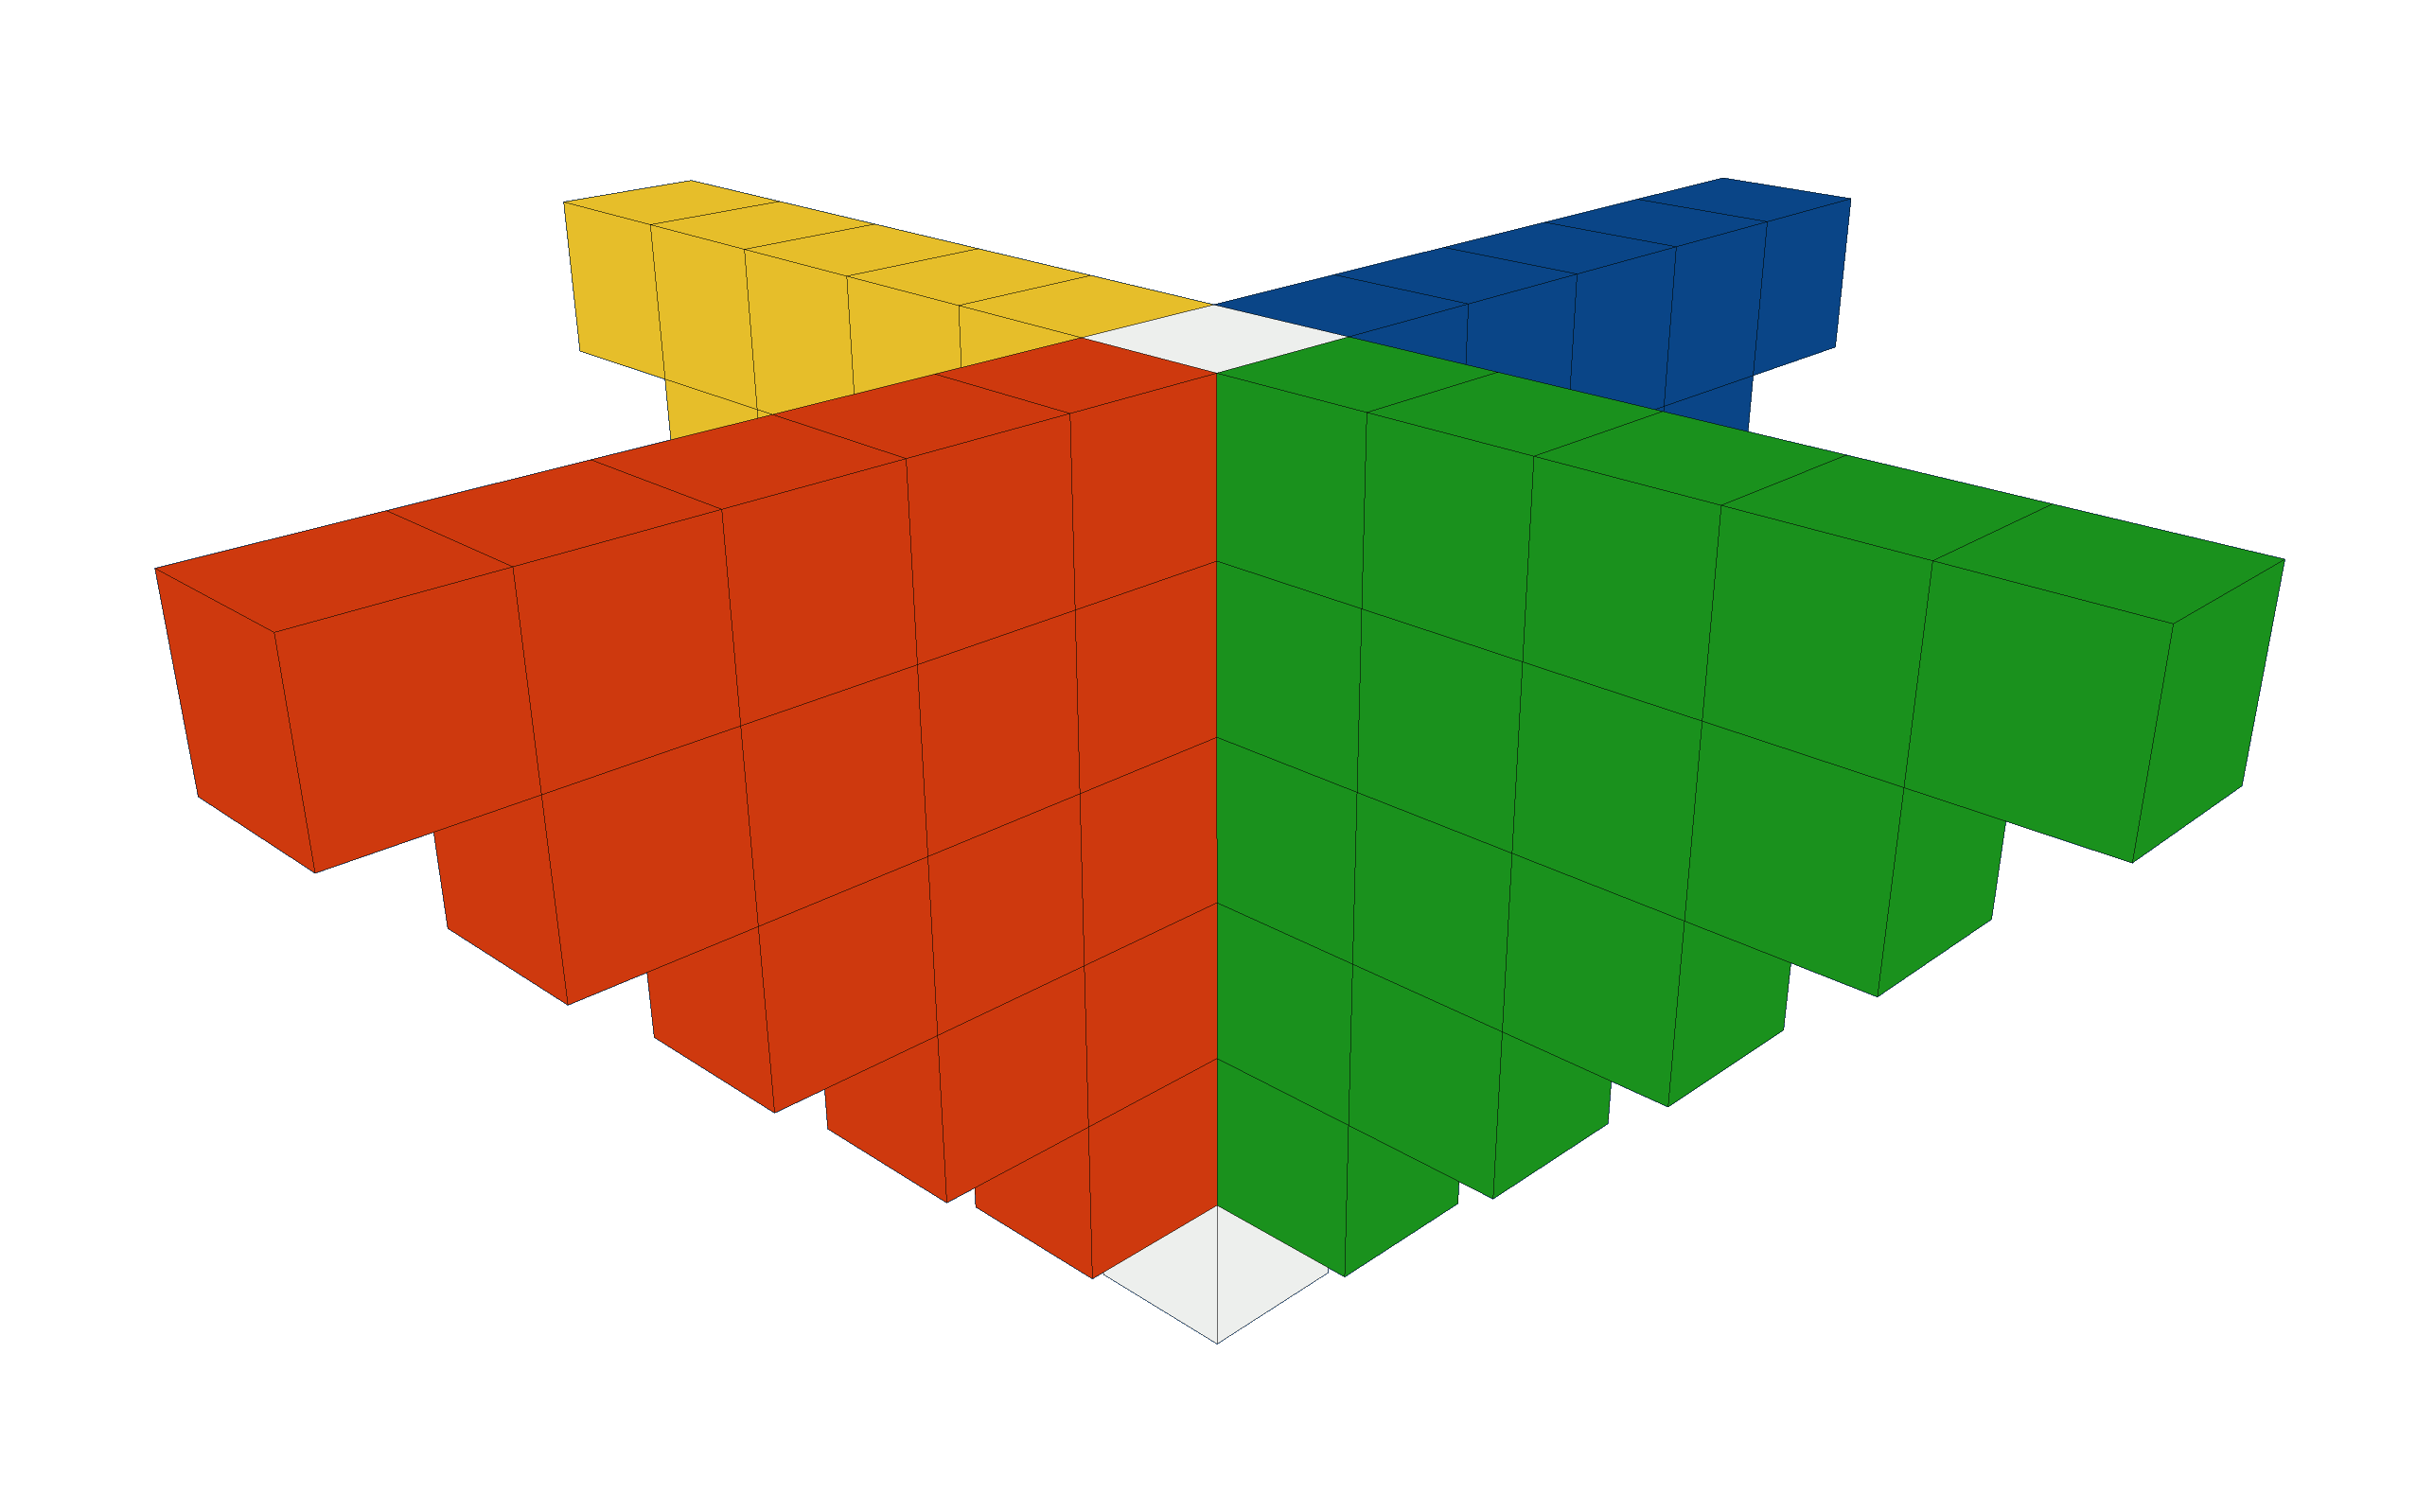
\includegraphics[height=0.063\textwidth]{../figures/angle1.png}\hspace{-5pt}
    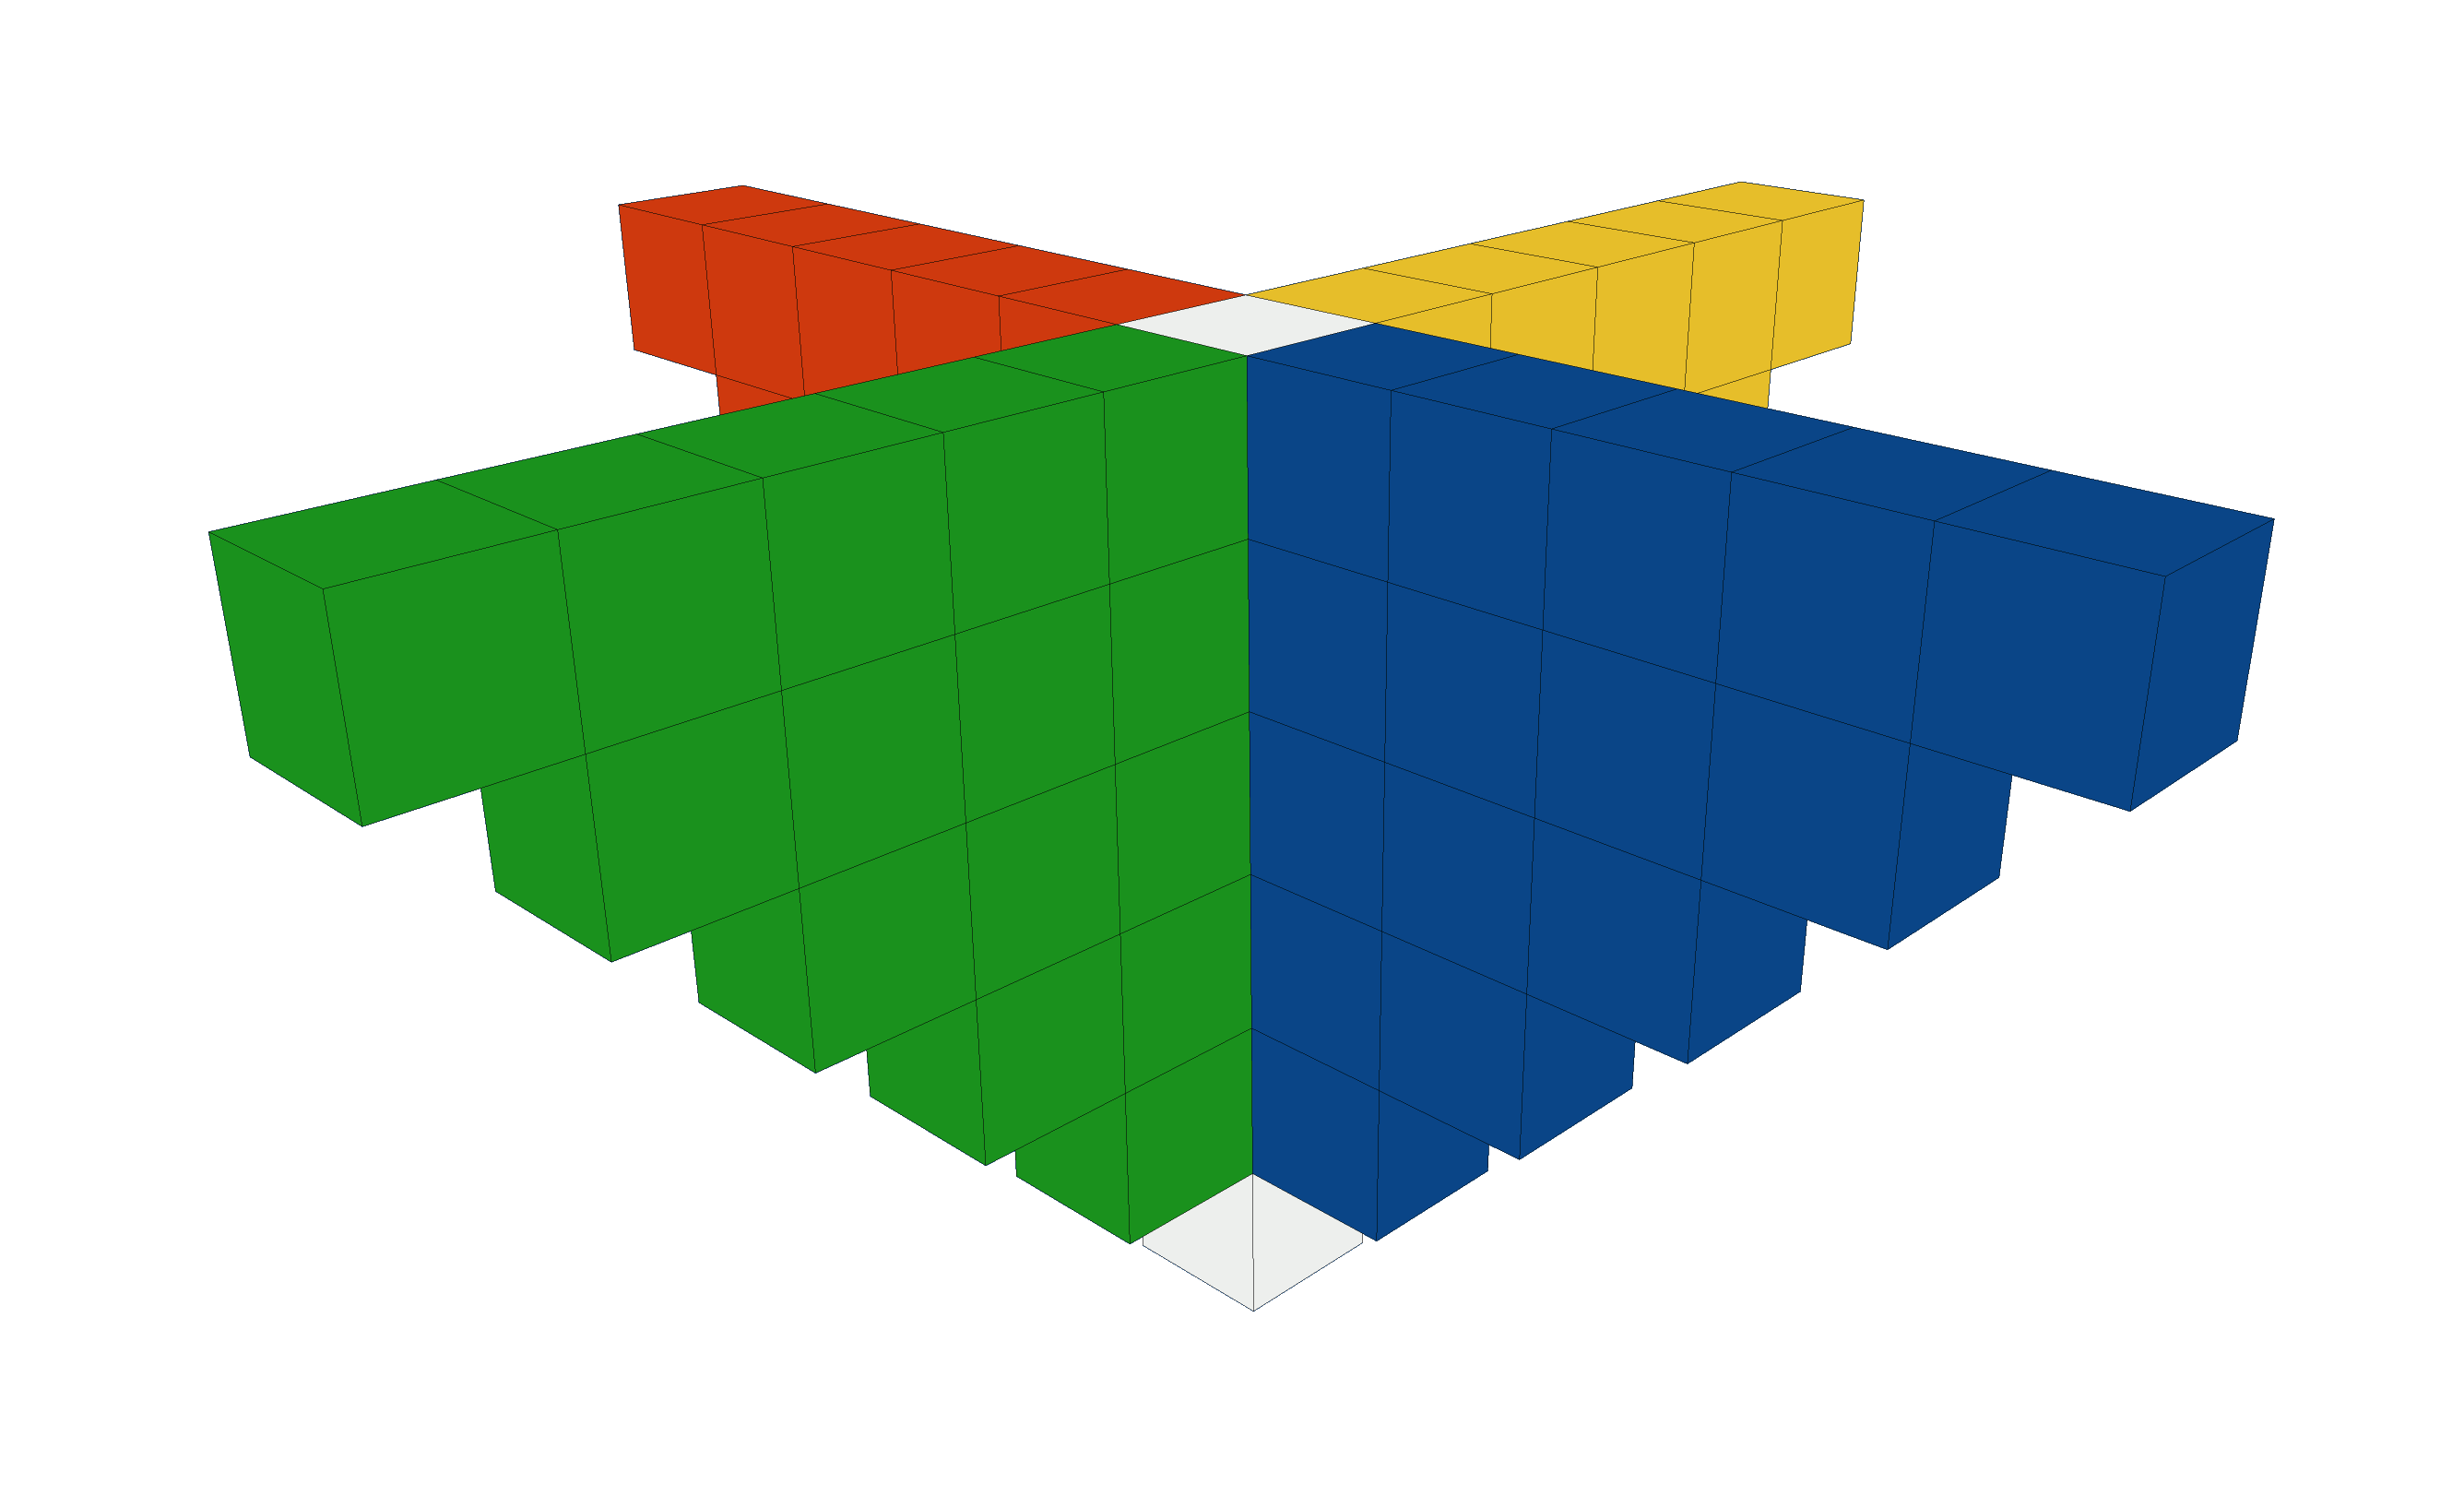
\includegraphics[height=0.063\textwidth]{../figures/angle2.png}\hspace{-5pt}
    
\includegraphics[height=0.063\textwidth]{../figures/angle5.png}\hspace{-5pt}
    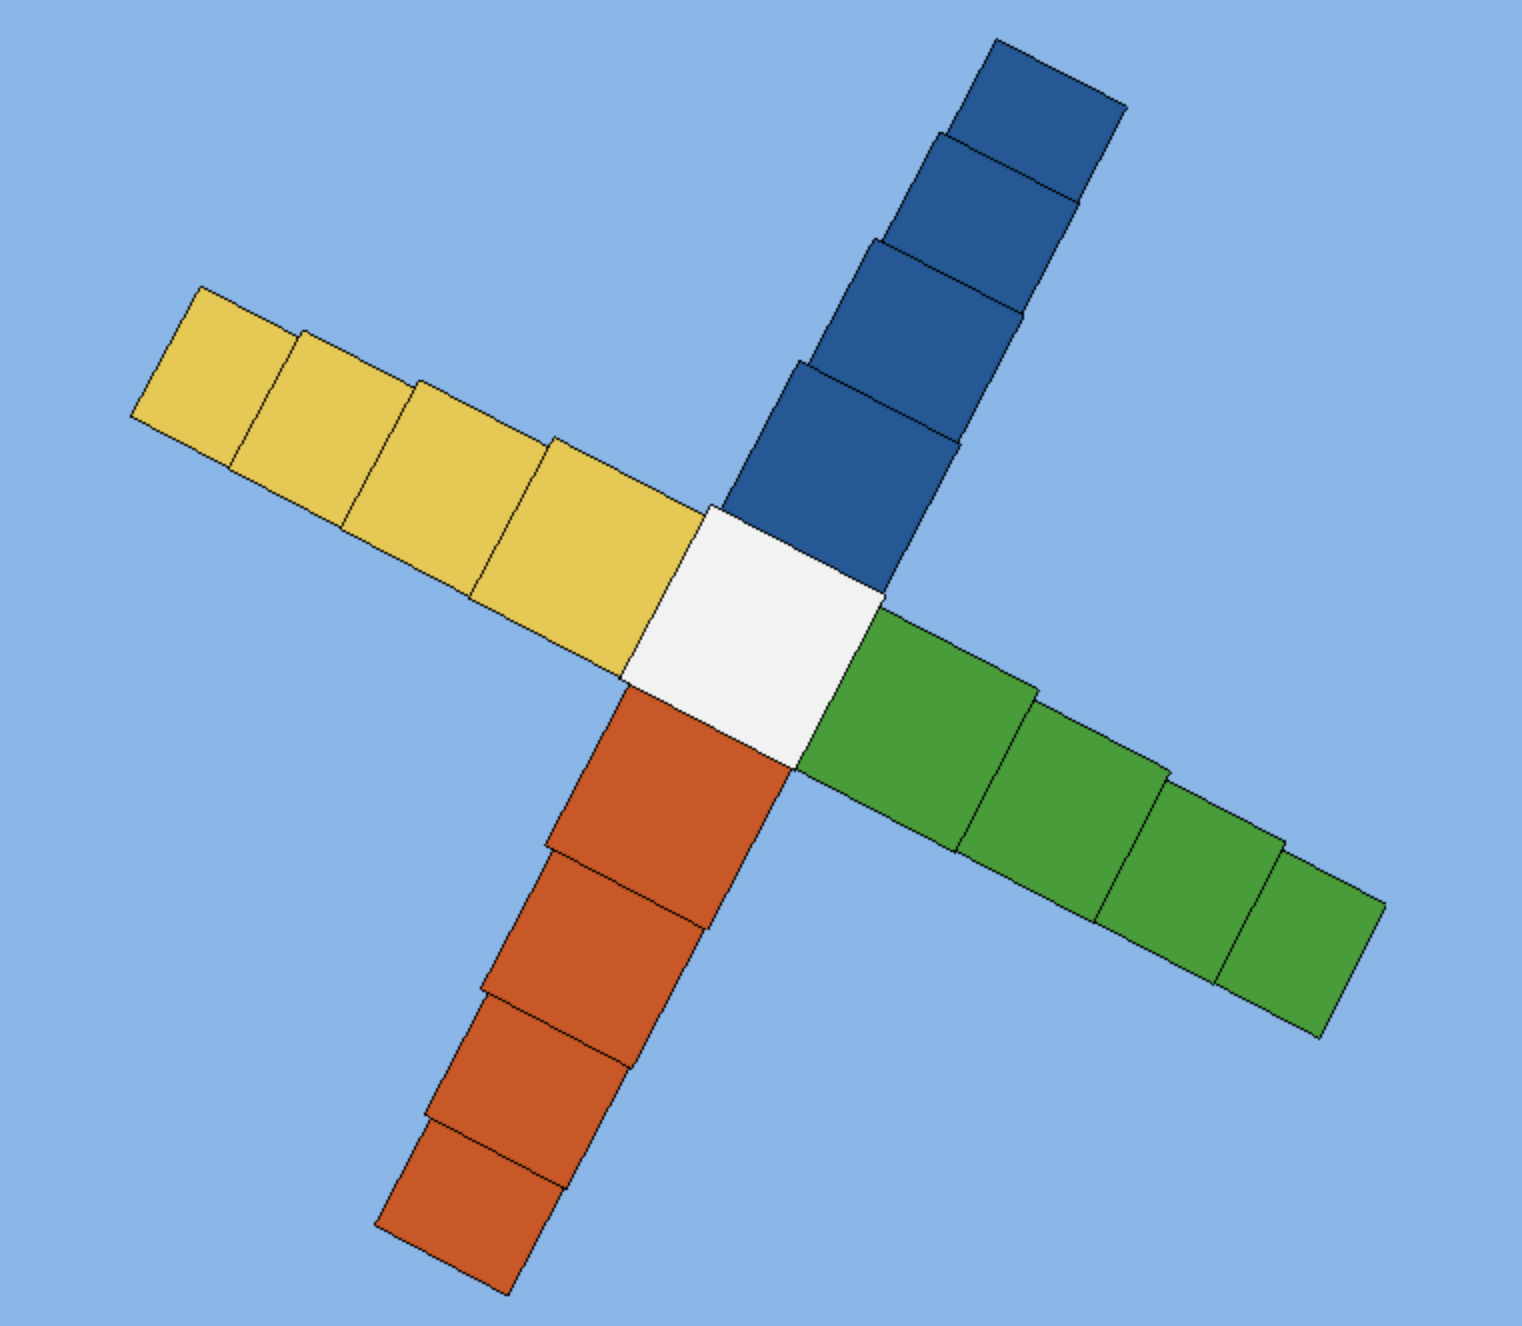
\includegraphics[height=0.063\textwidth]{../figures/angle3.png}\hspace{-3pt}
    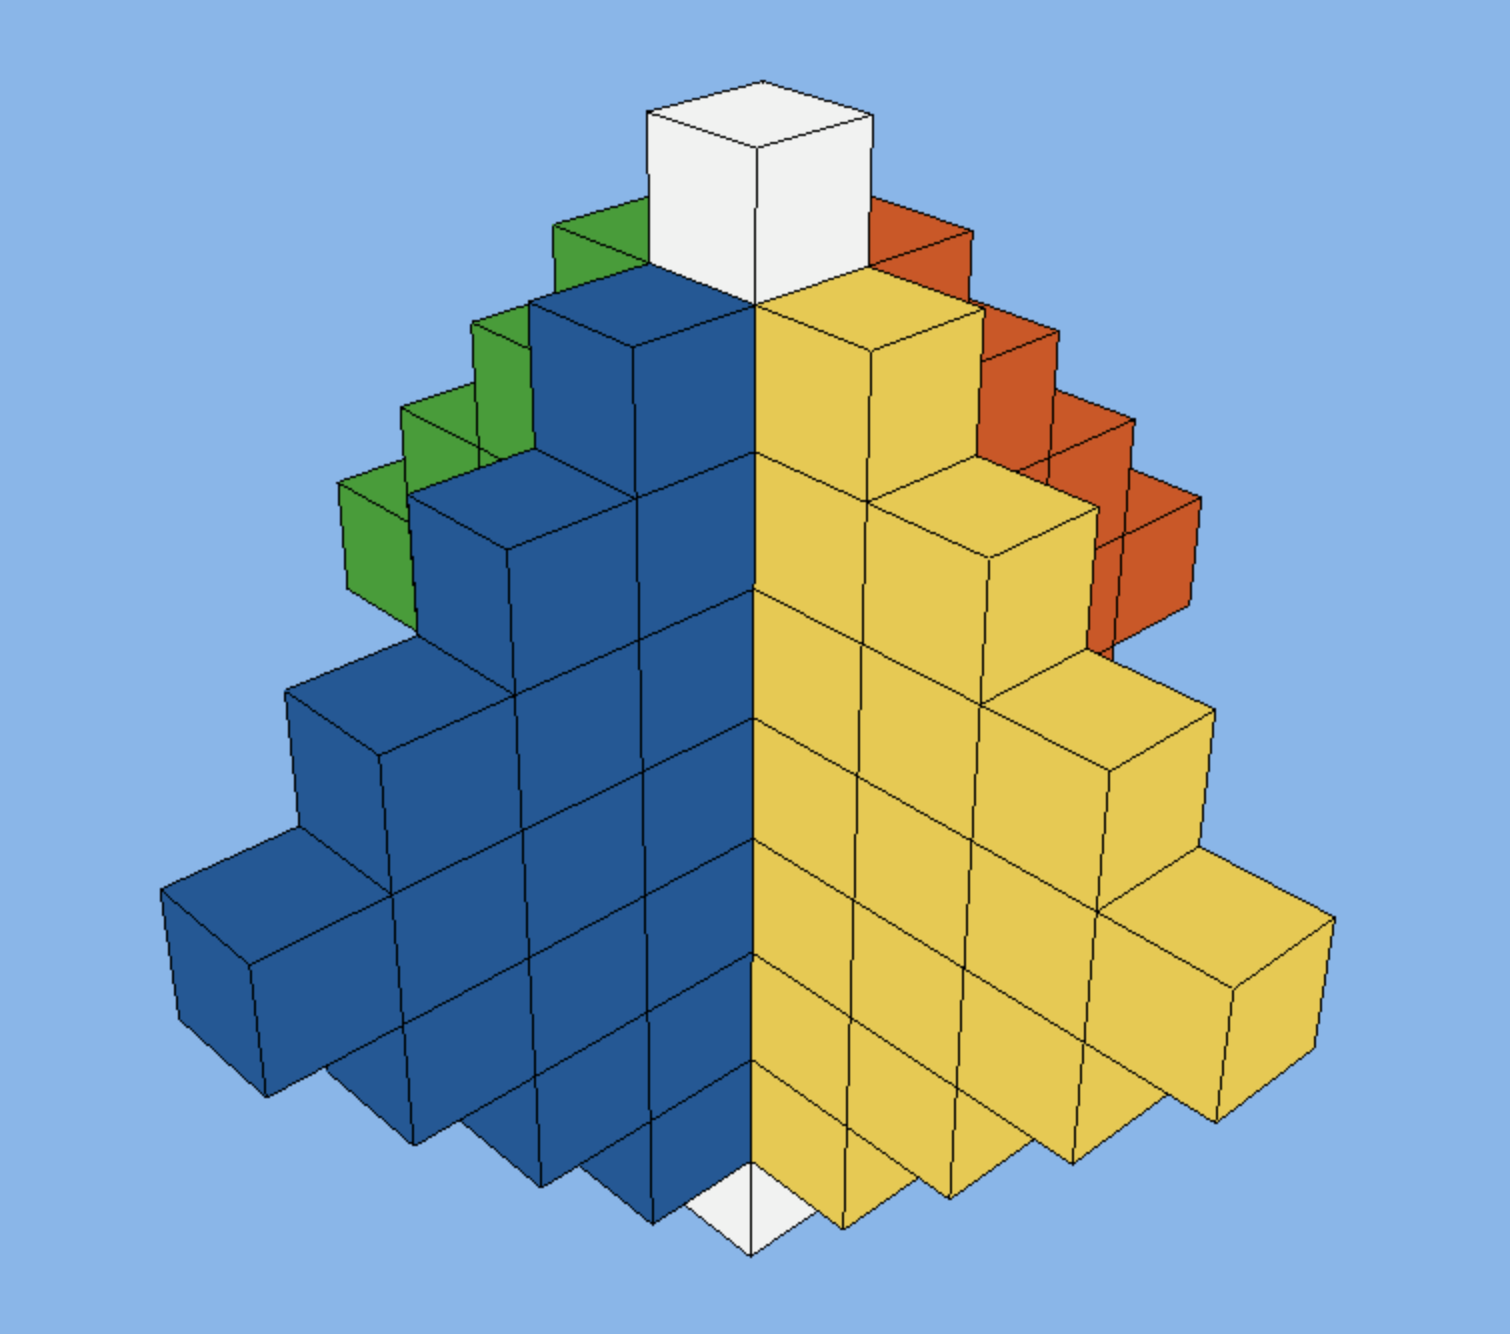
\includegraphics[height=0.063\textwidth]{../figures/angle4.png}
    \caption{Orientations of a $\bigcap_{i = 1}^4 \mathcal{L}(\mathcal{G}_i) \cap \Sigma ^6$ configuration. As $c \rightarrow \infty$, this shape approximates a circular cone whose symmetric axis joins $\sigma_i$ with orthonormal unit productions $w_i \rightarrow t_\cap$, and $S_i \in \Lambda^*_{\sigma}?$ represented by the outermost bitvector inhabitants. Equations of this form are equiexpressive with the family of CSLs realizable by finite CFL intersection.}
  \end{figure}

  \section{Levenshtein reachability}

  Levenshtein reachability is recognized by the nondeterministic infinite automaton (NIA) whose topology $\mathcal{L} = \knightkingarrow$ can be factored into a product of (a) the monotone Chebyshev topology $\kingarrow$, equipped with horizontal transitions accepting $\sigma_{i}$ and vertical transitions accepting Kleene stars, and (b) the monotone knight's topology $\knightarrow$, equipped with transitions accepting $\sigma_{i+2}$. The structure of this space can be finitely approximated by an acyclic NFA~\cite{schulz2002fast}, populated by accept states within radius $k$ of $q_{n,0}$, or equivalently, a left-linear CFG whose productions bisimulate the transition dynamics:

  \begin{figure}[H]
    \begin{minipage}[c]{0.45\textwidth}
      \centering
%      \underline{NFA}\vspace{10pt}
      \resizebox{0.8\textwidth}{!}{
      \begin{tikzpicture}[
%->, % makes the edges directed
      >=stealth',
      node distance=2.5cm, % specifies the minimum distance between two nodes. Change if necessary.
%  every state/.style={thick, fill=gray!10}, % sets the properties for each ’state’ node
      initial text=$ $, % sets the text that appears on the start arrow
      ]
      \node[state, initial]                (00) {$q_{0,0}$};
      \node[state, right of=00]            (10) {$q_{1,0}$};
      \node[state, right of=10]            (20) {$q_{2,0}$};
      \node[state, right of=20]            (30) {$q_{3,0}$};
      \node[right of=30]                   (40) {$\vphantom{\vdots}\cdots$};
      \node[accepting, state, right of=40] (n0) {$q_{n,0}$};

      \node[state, above of=00]            (01) {$q_{0,1}$};
      \node[state, right of=01]            (11) {$q_{1,1}$};
      \node[state, right of=11]            (21) {$q_{2,1}$};
      \node[state, right of=21]            (31) {$q_{3,1}$};
      \node[right of=31]                   (41) {$\vphantom{\vdots}\cdots$};
      \node[accepting, state, right of=41] (n1) {$q_{n,1}$};

      \node[above of=01]                   (0j) {$\mathmakebox[\widthof{$\cdots$}]{\vdots}$};
\node[right of=0j]                   (1j) {$\mathmakebox[\widthof{$\cdots$}]{\vdots}$};
\node[right of=1j]                   (2j) {$\mathmakebox[\widthof{$\cdots$}]{\vdots}$};
\node[right of=2j]                   (3j) {$\mathmakebox[\widthof{$\cdots$}]{\vdots}$};
\node[right of=3j]                   (4j) {$\iddots$};
\node[accepting, right of=4j]        (nj) {$\mathmakebox[\widthof{$\cdots$}]{\vdots}$};

\node[state, above of=0j]            (0k) {$q_{0,k}$};
\node[state, right of=0k]            (1k) {$q_{1,k}$};
\node[state, right of=1k]            (2k) {$q_{2,k}$};
\node[state, right of=2k]            (3k) {$q_{3,k}$};
\node[right of=3k]                   (4k) {$\vphantom{\vdots}\cdots$};
\node[accepting, state, right of=4k] (nk) {$q_{n,k}$};

\draw [->] (00) edge[below] node{$\sigma_1$} (10);
\draw [->] (10) edge[below] node{$\sigma_2$} (20);
\draw [->] (20) edge[below] node{$\sigma_3$} (30);
\draw [->] (30) edge[below] node{$\sigma_4$} (40);
\draw [->] (40) edge[below] node{$\sigma_n$} (n0);

\draw [->] (01) edge[below] node{$\sigma_1$} (11);
\draw [->] (11) edge[below] node{$\sigma_2$} (21);
\draw [->] (21) edge[below] node{$\sigma_3$} (31);
\draw [->] (31) edge[below] node{$\sigma_4$} (41);
\draw [->] (41) edge[below] node{$\sigma_n$} (n1);

\draw [->] (0j) edge[below] node{$\sigma_1$} (1j);
\draw [->] (1j) edge[below] node{$\sigma_2$} (2j);
\draw [->] (2j) edge[below] node{$\sigma_3$} (3j);
\draw [->] (3j) edge[below] node{$\sigma_4$} (4j);
\draw [->] (4j) edge[below] node{$\sigma_n$} (nj);

\draw [->] (0k) edge[below] node{$\sigma_1$} (1k);
\draw [->] (1k) edge[below] node{$\sigma_2$} (2k);
\draw [->] (2k) edge[below] node{$\sigma_3$} (3k);
\draw [->] (3k) edge[below] node{$\sigma_4$} (4k);
\draw [->] (4k) edge[below] node{$\sigma_n$} (nk);

\draw [->] (00) edge[left] node{$*$}         (11);
\draw [->] (10) edge[left] node{$*$}         (21);
\draw [->] (20) edge[left] node{$*$}         (31);
\draw [->] (30) edge[left] node{$*$}         (41);
\draw [->] (30) edge[bend right, below] node{$\sigma_5$} (41);
\draw [->] (40) edge[           right] node{$\sigma_n$}  (n1);
\draw [->] (40) edge[bend right, left] node{$*$}         (n1);

\draw [->] (01) edge[left] node{$*$}                     (1j);
\draw [->] (11) edge[left] node{$*$}                     (2j);
\draw [->] (21) edge[left] node{$*$}                     (3j);
\draw [->] (31) edge[left] node{$*$}                     (4j);
\draw [->] (31) edge[bend right, below] node{$\sigma_5$} (4j);
\draw [->] (41) edge[           right] node{$\sigma_n$}  (nj);
\draw [->] (41) edge[bend right, left] node{$*$}         (nj);

\draw [->] (0j) edge[left] node{$*$}                     (1k);
\draw [->] (1j) edge[left] node{$*$}                     (2k);
\draw [->] (2j) edge[left] node{$*$}                     (3k);
\draw [->] (3j) edge[left] node{$*$}                     (4k);
\draw [->] (3j) edge[bend right, below] node{$\sigma_5$} (4k);
\draw [->] (4j) edge[           right] node{$\sigma_n$}  (nk);
\draw [->] (4j) edge[bend right, left] node{$*$}         (nk);

\draw [->] (00) edge[bend left, left] node{$*$}   (01);
\draw [->] (10) edge[bend left, left] node{$*$}   (11);
\draw [->] (20) edge[bend left, left] node{$*$}   (21);
\draw [->] (30) edge[bend left, left] node{$*$}   (31);
\draw [->] (40) edge[right] node{$*$}             (41);
\draw [->] (n0) edge[bend right, right] node{$*$} (n1);

\draw [->] (01) edge[bend left, left] node{$*$}   (0j);
\draw [->] (11) edge[bend left, left] node{$*$}   (1j);
\draw [->] (21) edge[bend left, left] node{$*$}   (2j);
\draw [->] (31) edge[bend left, left] node{$*$}   (3j);
\draw [->] (41) edge[right] node{$*$}             (4j);
\draw [->] (n1) edge[bend right, right] node{$*$} (nj);

\draw [->] (0j) edge[bend left, left] node{$*$}   (0k);
\draw [->] (1j) edge[bend left, left] node{$*$}   (1k);
\draw [->] (2j) edge[bend left, left] node{$*$}   (2k);
\draw [->] (3j) edge[bend left, left] node{$*$}   (3k);
\draw [->] (4j) edge[right] node{$*$}             (4k);
\draw [->] (nj) edge[bend right, right] node{$*$} (nk);

\draw [->] (00) edge[below] node{$\sigma_2$}    (21);
\draw [->] (10) edge[below] node{$\sigma_3$}    (31);
\draw [->] (20) edge[below] node{$\sigma_4$}    (41);

\draw [->] (01) edge[below] node{$\sigma_2$}    (2j);
\draw [->] (11) edge[below] node{$\sigma_3$}    (3j);
\draw [->] (21) edge[below] node{$\sigma_4$}    (4j);

\draw [->] (0j) edge[below] node{$\sigma_2$}    (2k);
\draw [->] (1j) edge[below] node{$\sigma_3$}    (3k);
\draw [->] (2j) edge[below] node{$\sigma_4$}    (4k);

%https://tex.stackexchange.com/a/20986/139648
\draw [decorate,decoration={brace,amplitude=10pt,raise=10pt,mirror}] (00.south west) -- (n0.south east) node[midway,yshift=-3em]{\textbf{String length}};
\draw [decorate,decoration={brace,amplitude=10pt,raise=20pt}] (00.south west) -- (0k.north west) node[midway,xshift=-40pt,rotate=90]{\textbf{Levenshtein edit distance}};
\end{tikzpicture}
}
\end{minipage}
%\hfill
%\begin{minipage}[l]{5 cm}
%\centering
%\underline{CFG}\vspace{7pt}
%\begin{align*}
%S &\Rightarrow \{\cdot \in Q \mid \delta(\cdot, q_{n,0}) \leq k\}\\
%* &\Rightarrow \{\cdot \in \Sigma\}\\
%\big\{q_{i, j} &\Rightarrow \{q_{i, j-1}*\} \mid i, j \in [1, n]\times[1, k]\big\}\\
%\big\{q_{i, j} &\Rightarrow \{q_{i-1, j-1}*\}\mid i, j\in[1, n]\times [1, k]\big\}\\
%\big\{q_{i, j} &\Rightarrow \{q_{i-1, j} \sigma_i \}\mid i, j \in [1, n]\times[0, k]\big\} \\
%\big\{q_{i, j} &\Rightarrow \{q_{i-2, j-1} \sigma_i\} \mid i, j \in [2, n]\times[1, k] \big\}\\
%\end{align*}
%\end{minipage}
%\caption{Levenshtein reachability from $\Sigma^n$ can be described as either an acyclic $\epsilon$-free NFA, or a left-linear CFG.}
\end{figure}

%\noindent By intersection with a conjunctive language, we obtain a language $\mathcal{L}(\mathcal{G})$ that is both a subset of $\Sigma^n$ and accepted by $\mathcal{G}$. We can then define the Levenshtein reachability problem as follows: given a string $\sigma \in \Sigma^n$, find the smallest $k$ such that $\sigma \in \mathcal{L}(\mathcal{G})$.

%\begin{figure}[H]
%\begin{minipage}[c]{0.23\textwidth}
%\centering
%\resizebox{\textwidth}{!}{
%\begin{tikzpicture}[
%dot/.style = {circle, inner sep=0pt, minimum size=1mm, fill,
%node contents={}}
%]
%\def\firstcircle{(-2.1,0) coordinate (a) circle (2.4cm)}
%\def\firstcirclea{(-2.1,0) coordinate (b) circle (0.6cm)}
%\def\firstcircleb{(-2.1,0) coordinate (c) circle (1.2cm)}
%\def\firstcirclec{(-2.1,0) coordinate (d) circle (1.8cm)}
%\def\secondcircle{(1.2,0) coordinate (e) circle (1.5cm)}
%\begin{scope}
%\clip \secondcircle;
%\fill[black!15] \firstcircle;
%\end{scope}
%\draw \firstcircle node[dot,label=$\err{\sigma}$](z0);
%\draw [dashed] \firstcirclea;
%\draw [dashed] \firstcircleb;
%\draw [dashed] \firstcirclec;
%\draw[-stealth] (-2.1,0) -- (-1.5, 0) node[midway,below]{$d_1$};
%\draw[-stealth] (-1.5,0) -- (-0.9, 0) node[midway,below]{$d_2$};
%\draw[-stealth] (-0.9,0) -- (-0.3, 0) node[midway,below]{$\vphantom{d}\ldots$};
%\draw[-stealth] (-0.3,0) -- (0.3, 0) node[midway,below]{$d^*$};
%\draw[-stealth] (-0.3,0) -- (0.3, 0) node[midway,above]{$\tilde{\sigma}$};
%\draw \secondcircle;
%\node [above] at (current bounding box.north -| a) {$\mathcal{L}(G(\err\sigma, d^*))$};
%\node [above,yshift=1.5cm] at (e) {$\mathcal{L}(\mathcal{G}')$};
%\end{tikzpicture}
%}
%\end{minipage}
%\caption{LED is computed gradually by incrementing $d$ until $\mathcal{L}^\cap_{d}\neq \varnothing$.}
%\end{figure}

%  \subsection{Gradient estimation}
%
%  Given some unparseable string, i.e., $\squiggly{\sigma_1\ldots\:\sigma_n}: \highlight{\Sigma}^n \cap\mathcal{L}(\mathcal{G})^c$,\vspace{-4pt}\\where should we put holes to obtain a parseable $\sigma' \in \mathcal{L}(\mathcal{G})$? To estimate the effect of perturbing $\sigma$ on $\Lambda_\sigma^*$, one can either (1) backpropagate $\nabla S$ across upper-triangular entries of $\mathcal{M}^*$, or (2) stochastically sample \textit{minibatches} $\bm{\sigma}:\Sigma^{n\pm q}\sim\Delta_{q}(\sigma)$ from the Levenshtein q-ball centered on $\sigma$, i.e., the space of all edits with Levenshtein distance $\leq q$, loosely analogous to a finite difference approximation. Let us consider (2) and % This loosely corresponds to a finite difference approximation in $\mathbb{R}^n$.
%%  In other words, we seek:
%%
%%  \begin{align}
%%    \bigcup_{\bm{\sigma}\sim\Delta_{k}(\sigma)} \{\sigma' \in \bm{\sigma} \mid S \in \Lambda_{\sigma'}^*\}
%%  \end{align}
%
%
%  \noindent suppose $U: \mathbb{F}_2^{m\times m}$ is a matrix whose structure is shown in Eq.~\ref{eq:lfsr}, wherein $C$ is a primitive polynomial over $\mathbb{F}_2^m$ with coefficients $C_{1\ldots m}$ and semiring operators $\oplus := \veebar, \otimes := \land$:\vspace{-5pt}
%
%  \begin{align}
%    U^tV = \begin{pNiceMatrix}[nullify-dots,xdots/line-style=loosely dotted]
%                      C_1    & \cdd  &       &       & C_m \\
%                      \top   & \circ & \cdd  &       & \circ \\
%                      \circ  & \ddd  & \ddd  &       & \vdd \\
%                      \vdd   & \ddd  &       &       & \\
%                      \circ  & \cdd  & \circ & \top  & \circ
%    \end{pNiceMatrix}^t
%    \begin{pNiceMatrix}[nullify-dots,xdots/line-style=loosely dotted]
%      V_1 \\
%      \vdd\\
%      \\
%      \\
%      V_m
%    \end{pNiceMatrix}\label{eq:lfsr}
%  \end{align}
%
%  \noindent Since $C$ is primitive, the sequence $\mathbf{S} = (U^{0 \ldots 2^m-1}V)$ must be \textit{fully periodic}, i.e., for all ${i, j \in[0, 2^m), \mathbf{S}_i = \mathbf{S}_j \Rightarrow i = j}$. To uniformly sample $\bm\sigma \sim \Sigma^d$ without replacement, we form an injection $\mathbb{F}_2^m\rightharpoonup\Sigma^d$, cycle over $\mathbf{S}$, then discard samples which index any nonexistent element(s) of $\Sigma$. This method will reject $(1 - |\Sigma|2^{-\lceil\log_2|\Sigma|\rceil})^d$ samples overall, and requires $\mathcal{O}(1)$ per sample and $\mathcal{O}(|\Sigma|^d)$ to cover $\Sigma^d$. Next, to admit deletion, we augment $P$ with $(\varepsilon^+ \rightarrow \varepsilon \mid \varepsilon^+\:\varepsilon^+)$ and replace each production $(w \rightarrow t)$ with $(w \rightarrow t\:\varepsilon^+ \mid \varepsilon^+\:t \mid t)$. Finally, to generate $\bm{\sigma}\sim\Delta_{q}(\sigma)$, we enumerate hole configurations $H(\sigma, i) = \sigma_{1\ldots i-1}\:\text{\_ \_}\:\sigma_{i+1\ldots n}$ for each $i \in \stirlingii{n}{d}$ and $d \in 1\ldots q$, then solve for $\mathcal{M}^*$. If $S \in \Lambda^*_{\bm\sigma}?$ has at least one solution, each
%
%  \noindent edit in each $\sigma' \in \bm\sigma$ will match exactly one of seven patterns:\vspace{-10pt}
%
%  \begin{align*}
%    \text{Deletion}&=\begin{cases}
%    \sigma_{1}\:\ldots\:\text{\hlred{$\gamma_1$}\:\hlred{$\gamma_2$}}\:\ldots\:\sigma_n\hspace{0.2cm}\gamma_{1, 2} = \varepsilon\label{eq:del}
%    \end{cases}\\
%    \text{Substitution}&=\begin{cases}
%    \sigma_{1}\:\ldots\:\text{\hlorange{$\gamma_1$}\:\hlred{$\gamma_2$}}\:\ldots\:\sigma_n\hspace{0.2cm}\gamma_1 \neq \varepsilon \land \gamma_2 = \varepsilon\label{eq:sub1}\\
%    \sigma_{1}\:\ldots\:\text{\hlred{$\gamma_1$}\:\hlorange{$\gamma_2$}}\:\ldots\:\sigma_n\hspace{0.2cm}\gamma_1 = \varepsilon \land \gamma_2 \neq \varepsilon\label{eq:sub2}\\
%    \sigma_{1}\:\ldots\: \text{\hlorange{$\gamma_1$}\:\hlorange{$\gamma_2$}}\:\ldots\:\sigma_n\hspace{0.2cm}\{\gamma_1, \gamma_2\}\cap\{\varepsilon, \sigma_i\} = \varnothing \label{eq:sub3}
%    \end{cases}\\
%    \text{Insertion}&=\begin{cases}
%    \sigma_{1}\:\ldots\: \text{\hlgreen{$\gamma_1$}\:\hlorange{$\gamma_2$}}\:\ldots\:\sigma_n\hspace{0.2cm}\gamma_1 = \sigma_i \land \gamma_2 \notin \{\varepsilon,  \sigma_i\}\label{eq:ins2}\\
%    \sigma_{1}\:\ldots\: \text{\hlorange{$\gamma_1$}\:\hlgreen{$\gamma_2$}}\:\ldots\:\sigma_n\hspace{0.2cm}\gamma_1 \notin \{\varepsilon, \sigma_i\} \land \gamma_2 = \sigma_i\label{eq:ins1}\\
%    \sigma_{1}\:\ldots\: \text{\hlgreen{$\gamma_1$}\:\hlgreen{$\gamma_2$}}\:\ldots\:\sigma_n\hspace{0.2cm}\gamma_{1,2} = \sigma_i\label{eq:copy}
%    \end{cases}
%  \end{align*}
%
%\noindent This approach is tractable for $n \lesssim 100, q \lesssim 3$, however more complex repairs require a more efficient gradient estimator.

%  \noindent Eq.~(\ref{eq:del}) corresponds to deletion, Eqs.~(\ref{eq:sub1},~\ref{eq:sub2},~\ref{eq:sub3}) correspond to substitution, and Eqs.~(\ref{eq:ins1},~\ref{eq:ins2},~\ref{eq:copy}) correspond to insertion.

%  This constitutes to a top-down inference procedure, in which, following the tradition of Bird and Meertens, we define the exponential of a forest as a nested datatype called a \textit{taiga}:
%
%  \begin{align*}
%    \text{\textbf{data} \textit{Tree} } a &= \varnothing \mid \langle a, \langle\textit{Tree a, Tree a}\rangle\rangle\\
%    \text{\textbf{data} \textit{Forest} } a &= \varnothing \mid \langle \{a\}, \{\langle\textit{Forest a,  Forest a}\rangle\}\rangle\\
%    \text{\textbf{data} \textit{Taiga} } a &= \varnothing \mid \langle a, [\langle\textit{Taiga (Taiga a)}\rangle^2]\rangle
%  \end{align*}
%
%  This is needed because of the doubly-ambiguous nature of tree search: a single string may have a parse forest, and an incomplete string simultaneously occupies a superposition of possible parse forests. When we encounter two adjacent parse forests which cannot be joined, we know that either (1) the left derivation must change (2) the right derivation must change or (3) there must be a hole in the middle which joins the two together. When recursing over the state space, we must simultaneously consider all three possibilities.


%  Together with the uniqueness constraint this ensures that at least one representative of each equivalence class is included... (TODO).

%  Although emptiness for CSLs is, in general, undecidable, unsatisfiability corresponds to emptiness of bounded CSLs. Anyhow, since we are working with bounded-width CSLs, everything collapses down to finite languages, which are always closed. Thus, Bar-Hillel and other elegant constructions become trivial when so restricted. So we can use it to decide impossible substrings and other decision problems which are typically intractable in more general settings.

%Assume a hypothetical $\Phi(\mathcal{G}': \mathbb{G}, \err{\sigma}: \Sigma^*)\mapsto \tilde{\sigma}: \mathcal{L}(\mathcal{G}')$ which takes a CFG, $\mathcal{G}'$, generating an arbitrary nonempty CFL, and an unparseable string, $\err{\sigma}$, and which returns element(s) of $\mathcal{L}(\mathcal{G}')$ most similar to $\err{\sigma}$ according to their Levenshtein distance $\Delta(\err{\sigma}, \cdot)$.

Let $G(\err{\sigma}: \Sigma^*, d: \mathbb{N}^+) \mapsto \mathbb{G}$ be the construction described above accepting a string, $\err{\sigma}$, an edit distance, $d$, and returning a grammar that accepts the language of all strings within Levenshtein radius $d$ of $\err{\sigma}$. To find the language edit distance and corresponding least-distance edit(s), we must find the least $d$ such that $\mathcal{L}^\cap_d := \mathcal{L}\big(G(\err\sigma, d)\big) \cap \mathcal{L}(\mathcal{G}')$ is nonempty, i.e.: \linebreak (1) $\tilde{\sigma}\in\mathcal{L}(\mathcal{G}')$, and (2) $\Delta(\err{\sigma}, \tilde{\sigma}) \leq d^* \Longleftrightarrow \tilde{\sigma} \in \mathcal{L}\big(G(\err{\sigma}, d^*)\big)$, and (3) $\not\exists \sigma' \in \mathcal{L}(\mathcal{G}').[\Delta(\err{\sigma}, \sigma') < d^*]$.
To satisfy these criteria, it suffices to check $d \in (0, d_{\max}]$ by encoding the Levenshtein automata and the original grammar as a single polynomial, call it $\varphi_d[\cdot]$, then gradually introduce new accepting states at increasing radii until either (1) a satisfying assignment is found or (2) $d_{\max}$ is attained. Defined recursively,

\begin{equation*}
\varphi_{d+1} := \begin{cases}
\varphi\big[q_{\{i, j \mid n-i+j\leq 1\}} \subset \Lambda_{\tilde{\sigma}}^*\big(G(\err\sigma, d_{\max})\big)\big] & \text{if $d=1$, or}\\
\varphi_{d} \oplus \varphi\big[q_{\{i,j \mid n-i+j=d+1\}} \subset \Lambda_{\tilde{\sigma}}^*\big(G(\cdot, \cdot)\big)\big] & \text{otherwise.}%\text{if $d \leq \max(|\err{\sigma}|, \min_{\sigma \in \mathcal{L}(\mathcal{G}')}|\sigma|)$}.
\end{cases}
\end{equation*}

\noindent $\varphi$ will surely terminate in at most either the number of steps required to overwrite every symbol in $\err{\sigma}$, or the length of the shortest string in $\mathcal{L}(\mathcal{G}')$, whichever is greater.
%\noindent The function $\varphi_{d+1}(\mathcal{G}', \err{\sigma})$ is a realizer of $\Phi$.

\section{Conclusion}

  Not only is multilinear algebra over finite fields an expressive language for inference, but also a natural one for studying decision problems on formal languages themselves. Galois fields enjoy rich connections to algebraic complexity theory, and are particularly amenable to both SAT encoding and GPU acceleration. In this work, we illustrate a few applications for code completion and syntax repair in context-free and linear conjunctive languages. In the future, we plan to extend our method to stochastic grammars like PCFGs and HMMs.

\bibliography{../bib/acmart}
\end{document}